\documentclass[a4paper, 11pt]{article}
% URL format stuff
\usepackage[hyphens,spaces,obeyspaces]{url}
\usepackage{ragged2e}
\setlength\RaggedRightParindent{\parindent} % default value of this parameter is `0pt`
\RaggedRight 
% Rest of the packages
\usepackage{comment} % enables the use of multi-line comments (\ifx \fi) 
\usepackage{fullpage} % changes the margin
\usepackage{amsmath}
\usepackage{graphicx}
\usepackage{booktabs}
\usepackage{amssymb}
\usepackage{mathrsfs}
\usepackage{amsthm}
\usepackage{algorithm} % must read after hyperref
\usepackage{algorithmic}
\usepackage{framed}
\usepackage[sort,nocompress]{cite}
\newtheorem{theorem}{Theorem}
\newtheorem{corollary}{Corollary}
\newtheorem{lemma}{Lemma}
\usepackage{setspace}
\usepackage[toc,page]{appendix}
\usepackage{color}

\newcommand{\etal}{\textit{et al}.}
\newcommand{\ie}{\textit{i}.\textit{e}.}
\newcommand{\eg}{\textit{e}.\textit{g}.}
\newcommand{\iid}{\textit{i.i.d}.}
\newcommand{\prob}{\mathbb{P}}
\newcommand{\E}{\mathbb{E}}
\newcommand{\sign}{\mathbb{I}}

\newcommand{\jkcomment}[2]{{\color{red}#1}\marginpar{\color{red}\tiny#2 [JK]}}
\newcommand{\jacomment}[2]{{\color{blue}#1}\marginpar{\color{blue}\tiny#2 [JA]}}
\newcommand{\hpcomment}[2]{{\color{magenta}#1}\marginpar{\color{magenta}\tiny#2 [HP}}

\begin{document}
\title{
\begin{figure}[h]% use "t!" to force the float to start the float at top of page
    \centering
        
\includegraphics[keepaspectratio, width=0.3\textwidth]{images/KOAlogo.png} \\
        
\includegraphics[keepaspectratio, width=0.3\textwidth]{images/KOAbanner.png}
\end{figure}
A Decentralized Loyalty Program}
\author{John Alora, Justin Koh, Hayden Poe}
\date{}
\maketitle

%Abstract
\begin{abstract}
Merchants spanning across industries implement loyalty programs to incentivize brand faithfulness among consumers. However, current stand-alone loyalty programs have a flailing success rate retaining customers and fail to take full advantage of network effects that can be gained through cooperative alliances. Though current coalition loyalty programs attempt to solve this issue, they typically conglomerate among large entities in similar industries, alienating smaller businesses that provide complimentary services. These traditional loyalty programs are costly to maintain and the lack of customer participation makes one question if they are even worth while. Koalition addresses the problems found in traditional loyalty programs by leveraging blockchain technology to create an ecosystem that promotes free flow of points for consumers, offer marketing opportunities for merchants, and provide comprehensive data analytics for its users to make better informed decisions. As a stable coin, Koalition's native currency (KOA) allows for convenient accounting and promotes higher transaction rates. Koalition introduces consumers to a vast network of merchants under a unified, fungible, and utilitarian rewards currency through an ergonomic user interface. Koalition is the next-generation rewards currency, providing an agile, industry-grade, and decentralized solution and a frictionless experience to all users.
\end{abstract}

%Content
\pagestyle{plain}
\section{Background} \label{sec:background}

\subsection{Introduction}
Loyalty programs (LPs) have been implemented across the globe to develop brand loyalty by rewarding returning customers. However, current LPs fail to take full advantage of the network effects that can be gained by leveraging blockchain technology. These advantages include increasing customer loyalty, eliminating third party fees through disintermediation, providing data analytics through customer redemption patterns, and leveraging global integration to develop cooperative alliances that span industries and create a more functional LP for both consumers and merchants. 

Koalition is the next generation LP, creating a robust rewards network that integrates existing LPs and adds new opportunities for businesses that previously lacked the resources to deploy their own LP. This network of merchants provides more enticing incentives to customers by allowing them to spend their points when, where and how they want to.  Koalition enables customers to accumulate enough points to redeem for meaningful rewards without the hassle of managing separate accounts for dozens of LPs. For businesses, Koalition makes each rewards point transaction more secure and transparent, while removing trusted third party (TTP) services.

The next sections will first focus on the limitations and problems associated with current rewards programs. Then the utility of blockchain technology will be touched upon before describing how it can be used to disrupt the current loyalty industry. Furthermore, the unique aspects of Koalition's decentralized attributes, token stability and added benefits will be described in further detail along with a roadmap for future development. 

\subsection{Types of Loyalty Programs}

\subsubsection{Stand-Alone Loyalty Programs}

Customer loyalty is an asset that can be leveraged by both small businesses and big brands. Customers loyal to a particular brand are more likely to spread positive word of mouth, less likely to be swayed by competitors, and are less price sensitive. To better compete in a competitive industry, companies in industries ranging from airlines to supermarkets to local coffee shops create incentives using LPs. These programs offer consumers rewards points proportional to their purchases and allow consumers to accumulate points to redeem different types of rewards. Many companies use LPs to increase customer retention as the cost of acquiring new customers is much greater \cite{VR16}. However, with thousands of programs to choose from, consumers oftentimes are circumscribed by making the most economic travel decisions. According to the $2015$ Colloquy Loyalty Census, the average household belongs to nearly 29 different loyalty programs \cite{CQ15}. This perpetuates frustration because customers either pay high costs for similar services to remain loyal to one LP or they have points scattered among a myriad of LPs that they are unable to redeem for anything worthwhile. The end result is account inactivity and low redemption rates. In fact, the 2016 Bond Loyalty Report which queried 12,000 Americans and 7,000 Canadians about their 280 loyalty programs across various industries, found that only 50\% of them were active members of their respective programs. Of those 50\%, a fifth of them had never redeemed their points. Unredeemed rewards points create accounting liabilities for merchants in the form of unrealized revenues that cannot be absolved until they are redeemed. Furthermore, customer retention rates diminish for LP members who do not redeem their points. These customers are 2.7 times more likely to join a different program altogether \cite{Bond16}. 

Many customers have familiarized themselves with LPs through the travel industry, however, travel companies continue to lose market share to Online Travel Agencies (OTAs). OTAs like Priceline and Expedia act as a one-stop shop for consumers by consolidating the experience of individually booking a flight, hotel, and rental car into one platform. OTAs have their own LPs which give customers more choices (so customers can select the cheapest flight with minimal opportunity costs) and make it increasingly difficult for traditional stand-alone LPs to compete. Airlines, hotels, and rental car companies share up to 20\% of their revenues with OTAs and OTAs are projected to own 41\% of travel industry bookings by 2020 \cite{OTA17}.  Despite this fact, merchants still use OTAs because exiting this channel would result in a significant loss of marketing opportunities.  It is clear that merchants need an alternative loyalty program that provides enough customer flexibility to compete with OTAs, or continue giving up revenue.

\subsubsection{Coalition Loyalty Programs}
While the number of stand-alone LPs have grown, the challenges of these programs to consumers and businesses alike have caused many businesses to search for different LP schemes. Businesses have begun to participate in coalition LPs in an effort to provide customers rewards that can be earned and redeemed faster with greater flexibility across businesses. Most coalition LPs are formed through the agglomeration of existing stand-alone LPs and consist of either pairwise partnerships such as Amex-Uber or centralized partnerships like Starwood Hotels and Resorts (U.S.) and SkyTeam (international alliance). These coalitions help split liability among the participating merchants and partially solve some of the customer frustrations while still attempting to increase customer retention and engagement rates. Furthermore, coalition LPs promote the acquisition of new customers more easily than stand-alone LPs due to inter-company cooperation which favors cross-selling. It costs less to join a coalition LP than to establish a stand-alone program, and empirical evidence shows that businesses in coalition LPs achieve higher marketing performance \cite{VR16}. 

However, coalitions are often times limited in scope. Coalitions typically form among large entities in similar industries (\ie\ the many large hotel, airline, and rental car brands within the travel industry). These coalitions alienate small to medium cap businesses providing complimentary services, and hence fail to leverage the additional network benefits provided by adding these businesses. Furthermore, complex exchange rates and liability transfers between various LPs in a coalition require negotiations that consume unnecessary time and resources. While coalition LPs mark a step forward to fixing the problems that plague stand-alone LPs, these programs have a long way to go to improve customer loyalty and enhance the customer experience.

\subsection{Centralized Databases}
Databases are the primary means by which any digital data and applications are stored. At a high level, these databases consist of a hard drive or series of hard drives whose low level operations (\ie\ where data is stored) is managed by the operating system (Windows, Mac, Linux, etc). A SQL (Structured Query Language) server runs on top of the operating system and is responsible for how the data is accessed, organized, and used. These digital databases are typically centralized and managed by either the business or a TTP. Centralized databases are easy to maintain and simple to implement, but data stored in these databases can be easily manipulated (mutable) by both external and internal actors due to its centralized nature (\ie\ there is a single point of failure). Centralized databases also suffer from increased complexity and maintenance cost as the number of users increase. As users increase, the amount of data stored in the database increases, driving a need for more costly digital space, operational resources, and more IT personnel to manage the database. These problems are significantly magnified for applications that require the interchange and communication of data across different databases. These applications include the formation of consortiums or coalitions in which businesses pool their resources together to achieve a common goal. Generally, centralization introduces a significant amount of friction in these applications because it inhibits modularity (must give control to a central entity, making it difficult to change individual structure), interoperability (different technology, different data structures, etc) and inclusion (difficult, incurs a cost, or slow to add new businesses).

\subsection{The Blockchain}

\subsubsection{Overview}
Blockchain is a novel technology that can address many of the pitfalls of centralized databases. Blockchain can provide an open, distributed database of records acting as a public ledger of all transactions or digital events that have occurred between all participating entities. Essentially, it is a shared database that allows multiple users (who do not trust each other) to transparently and securely modify the database directly to reflect a state change or digital event. This is indeed revolutionary because it enables an ecosystem that distributes the cost and resources to manage and operate a database among all the participants, not just the businesses providing a service. Furthermore, due to the decentralization of the data, a blockchain makes it nearly impossible for external or internal actors to manipulate the data. Indeed, one of the key security features of a blockchain is immutability- once data is stored on the blockchain, it cannot be changed.
%
\begin{framed}
\begin{quote}
\textit{``If TCP/IP is the standard for secure information transfer, then blockchain is the standard for secure value transfer."}
\end{quote}
\end{framed}

Bitcoin \cite{BTC08}, the world's first renowned public blockchain, represents the first use case of blockchain technology by generating value through digital scarcity. In the Bitcoin framework, the exchange of the native cryptocurrency, Bitcoin (BTC), represents a unique transaction. More precisely, consider the following example where John sends 1 BTC to Justin, who subsequently sends 0.5 BTC to Hayden. For simplicity, let us assume that John has 1 BTC in his account, while Justin and Hayden have 0 BTC in theirs. If John sends Justin 1 BTC, John signs a new transaction agreement that deducts 1 BTC from John?s account. This transaction agreement is now worth 1 BTC, and can only be spent by Justin. The transaction agreement between John and Justin (call this $T_1$) is now used to fund this transaction. Justin signs two transaction agreements: one transaction agreement that subtracts 0.5 BTC from $T_1$ and a second transaction agreement (call this $T_2$) with Hayden that is worth 0.5 BTC, which Hayden can spend immediately after the transaction is verified. Thus, in the Bitcoin use case, the blockchain is simply a ledger of unique transactions.

The security foundations of blockchains rely on asymmetric cryptography and distributed consensus \cite{PR17}. Each transaction agreement in the blockchain is protected with a digital signature. John uses his private key to sign the transaction agreement worth 1 BTC with Justin. Justin, using his public key, is then able to independently verify from the digital signature that John authorized the transaction. This prevents a malicious participant from forging a transaction involving John's assets because (s)he must have John?s private key. This transaction (and the transaction between Justin and Hayden) is broadcasted to every participant in the blockchain network in order to be validated and recorded. Transactions are ordered by placing the validated transactions into blocks. These blocks are then linked together to form a chain (hence blockchain) preserving a proper linear, chronological order. For example, the transaction between John and Justin ($T_1$) will always precede the transaction between Justin and Hayden ($T_2$) because any attempts to include $T_2$ in a block where $T_1$ does not precede $T_2$ will be rejected during the validation process (since Justin only has enough BTC to send to Hayden, if John sends it to him first). Note that since every participant is able to manage the blockchain, multiple blocks can be generated by different participants at the same time. In the Proof-of-Work (PoW) scheme, the first participant to solve an extremely difficult cryptographic puzzle will be able to submit their block to the blockchain provided that they prove to everyone in the network that they solved the puzzle. The process of validating the block and the participant's proof that (s)he solved the puzzle forms the consensus portion of the blockchain. Since everyone has the same version of the truth (i.e. same blockchain), it is impossible to change the contents of any block of the chain without getting caught. Furthermore, the difficulty of solving the cryptographic puzzle prevents one person from adding a false block to the chain. Figure \ref{fig:btcfigure} shows a general overview of how blockchains work.
%
\begin{figure}[] % use "t!" to force the float to start the float at top of page
    \centering
        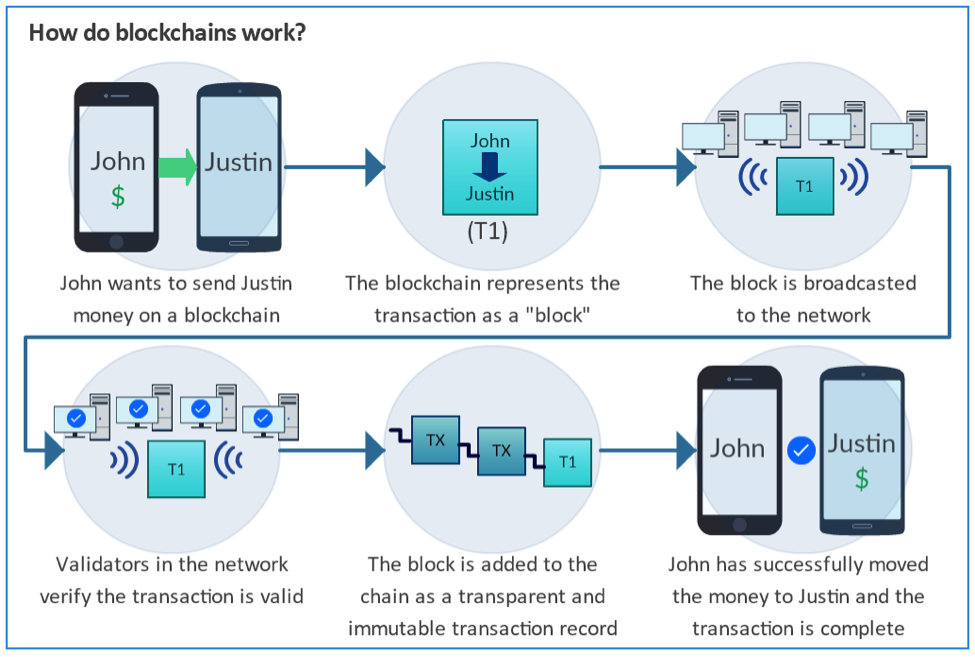
\includegraphics[keepaspectratio, width=0.7\textwidth]{images/blockchains.png}
    \caption{Overview of How Blockchains Work} \label{fig:btcfigure}
\end{figure}

The advent of Bitcoin has helped spawn more advanced blockchain-based platforms. Ethereum \cite{Wood14} is one of these platforms, which allows the implementation of so called smart contracts-- computer programs that control digital assets on the blockchain through a set of arbitrary rules. Smart contracts allow for the complete automation of processes requiring a TTP such as trade agreements, crowdfunding, and redemption of loyalty points. Decentralized applications (Dapps) are client-side applications that allow participants in the blockchain to interact with smart contracts. Dapps and smart contracts enable a dynamic environment for the interaction between participants on the network. %Figure \ref{fig:dapps} illustrates the interaction between Dapps and smart contracts.
%
%\begin{figure}[h] % use "t!" to force the float to start the float at top of page
%    \centering
%        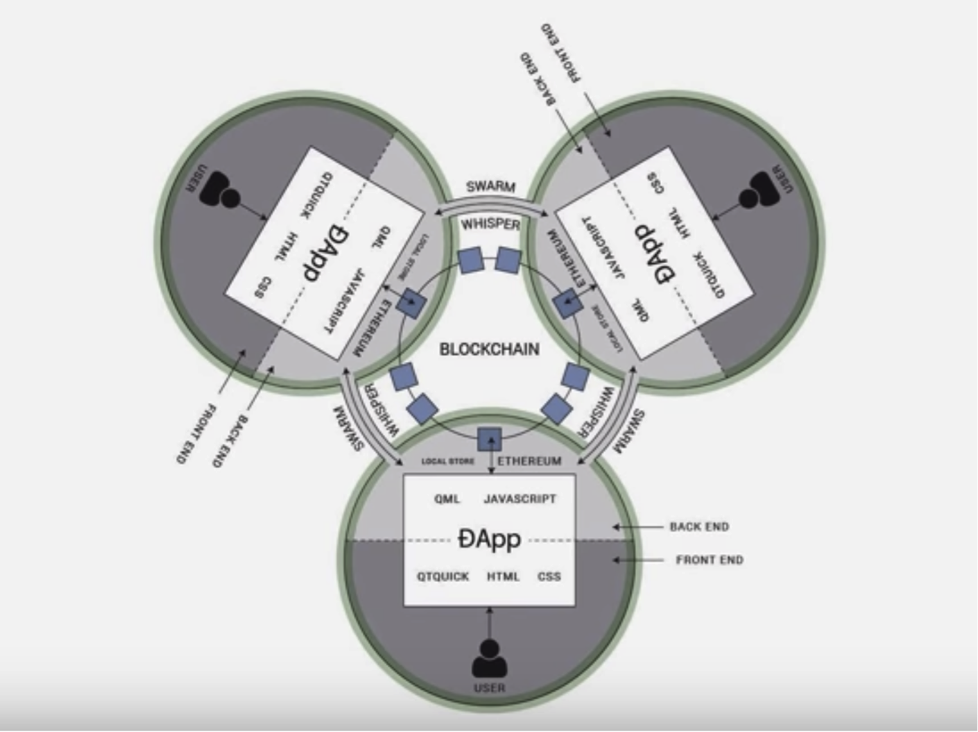
\includegraphics[keepaspectratio, width=0.7\textwidth]{images/dapps.png}
%    \caption{Interaction between Dapps and Smart Contracts} \label{fig:dapps}
%\end{figure}

Blockchains have seen tremendous growth since the introduction of Bitcoin, and the technology's development has accelerated due to increased adoption by startups and industry alike. For example, the Ethereum project continues to grow as it attempts to solve industry concerns about scaling, customer privacy, and regulation. Alternative blockchain-based platforms such as IBM's Hyperledger Fabric \cite{HL16}, Microsoft's Coco Framework \cite{Coco17}, Multichain \cite{MC16}, and NEM \cite{NEM} address the problem of scaling and customer privacy through permissioned or private blockchains. While these platforms handle a narrower range of use cases, they address some of the major problems raised by industry. Projects, such as Cardano \cite{Cardano}, aim to solve these problems while preserving the complexity of applications that can be run on the blockchain.

\subsubsection{Permissionless vs. Permissioned Blockchains}

The key design consideration for any blockchain-based protocol is whether to use a permissionless (e.g. Ethereum and Bitcoin) or a permissioned (e.g. Hyperledger Fabric and Multichain) blockchain. In a permissionless blockchain, chain consensus is achieved by all the users running the protocol, compared to a permissioned blockchain, where consensus is done by a small set of trusted users. While permissionless blockchains have high a degree of decentralization, the development of permissioned solutions was a response to the failure of existing, permissionless blockchains to meet several key requirements: high transaction throughput, confidentiality, and computational efficiency \cite{Vitalik15}. Furthermore, the cryptocurrencies of protocols in permissioned blockchains are not subject to speculation in the open market, establishing them as strictly functional assets in the protocol. There is a limited tradespace between these variables that an existing public blockchain may fail to support, hence, many companies have chosen to adopt permissioned blockchains. Table \ref{table:blockchaintypes} summarizes each of the two platforms' characteristics.
%
\begin{table}[h]
\centering
 \begin{tabular}{|c | c | c |} 
 \hline
  &  Permissionless Blockchain & Permissioned Blockchain \\ 
 \hline
 Throughput & Low & High  \\
 \hline
 Latency & Low & Medium \\
 \hline
 Number of Readers & High & High \\
 \hline
Number of Writers & High & Low \\
 \hline
 Centrally Managed & No & Yes \\
 \hline
\end{tabular}
\caption{Differences Between Permissionless and Permissioned Blockchains} \label{table:blockchaintypes}
\end{table}

While permissioned blockchains are regarded as an industry solution, permissionless blockchains enjoy first mover's advantage in terms of community and development maturity. In fact, many permissioned blockchains draw insights from Ethereum's open-source development and some, such as J.P. Morgan's Quorum \cite{Quorum16}, have even built permissioned platforms on top of the project's code base. Also, the community of these existing platforms (such as Bitcoin and Ethereum) as well as communities of newer projects (such as Cardano) are providing elegant solutions for most, if not all, of industry's concerns. Concerns regarding lack of confidentiality and computational efficiency in permissionless blockchains are also being addressed. Implementation of zero-proof knowledge will allow for confidential transaction of metadata on the blockchain. Off-chain execution of smart contracts (\eg\ Bitcoin's Lightning Network \cite{Poon16}) will reduce computation on the blockchain while enabling efficient micro-transactions. Transition from Proof-of-Work to the Proof-of-Stake (PoS) consensus mechanism (Ethereum's Casper \cite{Vitalik17} and Cardano's Ouroboros \cite{Kiayias17}) will reduce the required computational resources for chain consensus. In light of these developments, while permissioned blockchains seem to currently have an advantage over the permissionless platforms, this technological gap will close in the near future. Accounting for the fact that the biggest public blockchains have active communities that perpetuate the growth and development of their respective platforms, it is clear that that this gap will close rapidly and permissionless blockchains will become the industry-standard. 

%With Koalition?s vision of the protocol?s features in mind (see Section II), the flowchart in Figure 3 from Wust and Gervais? ?Do You Need a Blockchain?? was used to determine which blockchain platform to adopt [21].

\subsection{Blockchaining Loyalty} \label{sec:BCloyalty}
The widespread variety of LPs that are available to consumers has created a disorganized multi-currency environment. This environment is characterized by cumbersome exchange rates among partners, fragmented points collection among consumers, and limited marketing opportunities, effectively inhibiting customer experience and company profitability. This flailing ecosystem is what drives account inactivity and low redemption rates in LPs across all industries. As it stands, LPs are ripe for a disruptive protocol that makes them easier to use. The Koalition protocol would enable a fluid, interoperable environment where points are easily transferred and redeemed (frictionless), enable rapid addition of new partners without increasing complexity (inclusion), and enable more sophisticated cooperative marketing strategies that allow companies to generate even more incremental share.

Blockchain is the technology poised to be the foundation for this protocol \textbf{[16][17][18]}. By nature, centralized databases and TTPs introduce friction by limiting interoperability and inclusion. Implementation of a fluid and interoperable LP environment using centralized solutions is not scalable due to the tremendous amounts of complexity and cost required. Blockchain solves this scalability problem because it is a distributed database with multiple non-trusting writers that enables complex interactions of transactions. In other words, it enables an environment where participants can transact with each other freely and securely, while managing the protocol that enables this, all without an intermediary. Koalition envisions a LP protocol with the following features:
%
\begin{itemize}
\item{Frictionless transfer and redemption of LP-specific points on a single platform using a unicurrency.}
\item{Enhanced customer experience by easing management of LPs through a universal rewards wallet.}
\item{Increased inclusion by enabling the seamless addition and maintenance of loyalty partnerships.}
\item{Reduced merchant liability by increasing redemption options and unlocking inherent value of points.}
\item{Increased marketing opportunities through greater consumer data fidelity and more complex data analytics.}
\item{More sophisticated LP schemes that cater to the wants and needs of customers.}
\item{Volatility control will increase transactional value by removing asset speculation through token value stability.}
	\begin{itemize}
	\item{This eliminates a major concern faced by deflationary cryptocurrencies by encouraging the redemption of tokens as opposed to using it solely as an investment asset.}
	\end{itemize}
\end{itemize}

\subsubsection{A Permissionless Blockchain Solution to Loyalty}

This section justifies why a permissionless blockchain as a platform for loyalty programs is the best solution. As part of the discussion, a flowchart developed by Wust and Gervais in \cite{} is used (refer to Figure \ref{fig:decisionchart}). The purpose of the flowchart is to determine whether a blockchain is warranted for a specific use case and if so, what type. As discussed earlier, adoption of a blockchain-based solution mitigates the complexity and cost of centralized (and hence TTP) solutions, enabling a rich LP environment that promotes frictionless transactions, inclusion, and interoperability. Based on this, the first three steps in the flowchart are fulfilled, leading to the key design question: are all writers known? It turns out that by allowing all writers to not be known, a blockchain LP can be positioned for the future to scale as the number of users increase. More precisely, as the major public blockchains introduce parallel task execution (\ie\ sharding) and data compression, throughput will increase as more participants join the network. This is highly desirable as it promotes further network growth and disintermediation-- the participants who use the database, manage the database. This is the opposite of the current state of the art, where increasing network effects in permissionless blockchains reduces throughput and increases latency (see Table \ref{table:blockchaintypes}). While the current lack of scalability has driven companies to prefer permissioned blockchains, in order for a blockchain LP protocol to scale in the future it must first be implemented on a permissionless blockchain. 

Permissionless blockchains like Ethereum and NEM already have ready-to-use infrastructure with significant developer communities which eliminates the need to create a brand new platform.  This is not the case with most permissioned chains that require significant infrastructure development just to ensure consensus. Furthermore, permissionless blockchains already have many active users \textbf{expand this}.
%
\begin{figure}[t!] % use "t!" to force the float to start the float at top of page
    \centering
        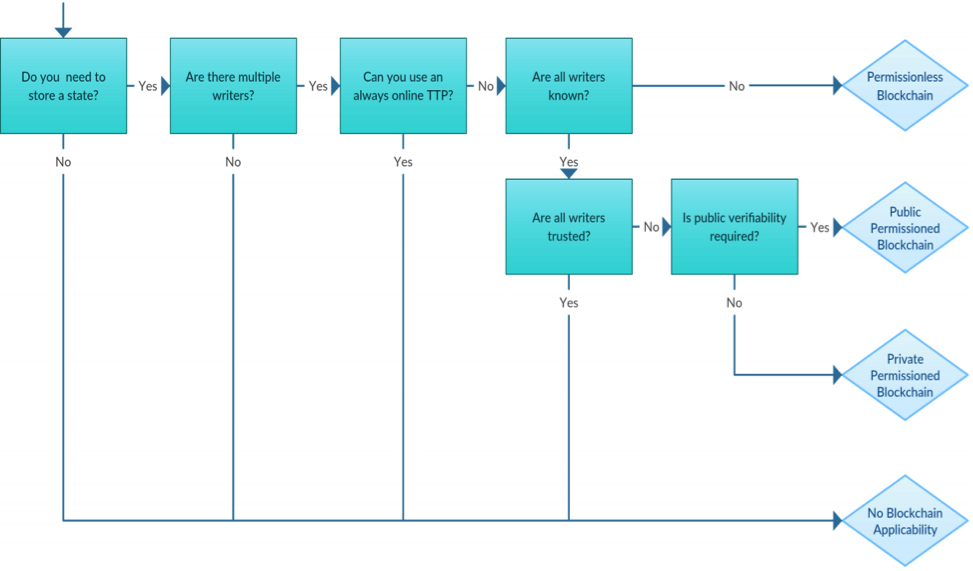
\includegraphics[keepaspectratio, width=0.7\textwidth]{images/decisionchart.png}
    \caption{``Do You Need a Blockchain?" Decision Flow Chart} \label{fig:decisionchart}
\end{figure}

\subsection{Cryptocurrency Price Stability}
The extreme price volatility of cryptocurrencies poses a main challenge for their widespread adoption. This volatility is a result of the nascent market's highly speculative nature driven by the market's expectation of substantial demand in the future. Speculation in coin demand translates to change in coin price, making price volatility proportional to demand volatility. Furthermore, the inelastic coin supply schemes adopted by most cryptocurrencies do nothing to dampen the effect of change in coin demand on the coin's price. This is a well-known problem and Satoshi Nakamoto (the inventor of Bitcoin) himself has admitted to the inadequacy of an inelastic supply in meeting rising demand \cite{Satoshi08}.
%
\begin{framed}
\begin{quote}
\textit{``The fact that new coins are produced means the money supply increases by a planned amount, but this does not necessarily result in inflation. If the supply of money increases at the same rate that the number of people using it increases, prices remain stable. If it does not increase as fast as demand, there will be deflation and early holders of money will see its value increase."}
\end{quote}
\end{framed}

As blockchain becomes more mainstream, there has been a greater urgency within the community to develop cryptocurrencies that are more price stable. These so called \textit{stable coins} attempt to peg their value to a more stable asset, such as a fiat currency, and are becoming more prominent. These stable coins fall into one of three main stabilization schemes: fiat-collateralized, crypto-collateralized, and non-collateralized. 

Fiat-collateralized stable coins are conceptually easy to understand: every one stable coin is redeemable for \$1. In other words, a user must deposit \$1 into the stable coin's fiat bank account in order for the stable coin's treasury to mint and issue one stable coin to the user. Whenever the user liquidates their stable coin for fiat, the treasury will destroy their stable coin and the user will be wire transferred the equivalent fiat. The benefits of this scheme is that it is completely price stable as  each stable coin is backed by 1 unit of fiat currency and is the simplest to implement. Its drawbacks are that it is centralized, expensive to maintain (due to high regulation and frequent audits), and is constrained by legacy payment rails. Tether \cite{Tether16} is an example of a fiat-collateralized stable coin and has done well in maintaining a peg to the USD.

Crypto-collateralized stable coins such as BitShare's BitUSD \cite{BTS15} and MakerDao's Dai \cite{MDao17} are similar to fiat-collateralized schemes except that collateral is held in another cryptocurrency instead of fiat. Since the collateral is a cryptocurrency that also experiences price volatility, these schemes require over-collateralization of the stable coin in order to absorb price fluctuations. Take the following example.
%
\begin{quote}
Hayden must deposit \$100 worth of Ether in order to be issued 50 \$1 stable coins. If the price of Ether drops 25\%, Hayden's remaining Ether collateral worth \$75 will still be able to back the price of each stable coin to \$1 each. If Hayden sells his 50 stable coins to John for \$50 in Ether, and John chooses to liquidate the 50 stable coins, then the treasury will give John \$50 in Ether and Hayden the remaining collateral of \$25 worth of Ether.
\end{quote}
%
As an incentive for the stable coin issuers, these schemes pay out interest to those who pay the necessary collateral to issue stable coin. While this scheme works great in a bull market, its ability to absorb significant price declines in the underlying crypto-collateral is limited by the amount of over-collateralization required by the scheme. If the crypto-collateral price drops significantly, there may not be enough collateral to back the price of the stable coin. In these cases, crypto-collateralized schemes will automatically liquidate and destroy users' stable coin for their underlying collateral. So while crypto-collateralized schemes are more decentralized and are able to quickly liquidate their stable coin into the underlying collateral, these schemes are less price stable, more complex, and are more inefficient with respect to use of capital than fiat-collateralized schemes. 

Instead of pegging a stable coin to its collateralized assets' price, non-collateralized stable coins utilize an algorithmic treasury (via smart contract) that has a singular monetary policy--ensure the stable coin trades at a fixed fiat price. This scheme borrows ideas from the \textit{Hayek Money} approach proposed by Ametrano in \cite{Hayek16} which advocates for an elastic supply and a protocol that rebases wallet balances proportional to the change in stable coin price. Non-collateralized stabilization schemes also have some semblance of buffer stock schemes--a program that stores a certain amount of commodity when the price is low, and to release a certain amount of the stored commodity when the price is high. Buffer stocks are well-studied (see \cite{An13}) and \cite{Ath08} and have been widely used in developing countries to to help stabilize food prices and ensure food security. The merging of these two concepts combined with a new scheme called \textit{Seigniorage Shares} by Robert Sams \cite{Sams15} has served as the foundation for non-collateralized stabilization schemes. The idea behind non-collateralized stable coins is simple: as the price of the stable coin increases, the smart contract will mint new coins and auction them out to the market until the price goes back to the desired price. The \textit{seigniorage} gained from this period will be used to buy back coins in the market to reduce supply and drive prices up. If the collected seigniorage is insufficient to buy up enough coins, the Seignorage Shares approach calls for the treasury smart contract to issue shares that entitle users (who are willing to liquidate their stable coin) to future seigniorage. The biggest challenges with non-collateralized stable coins are that it requires continual growth and is difficult to analyze with respect to safety margins for the seigniorage pool. Along with these challenges are characteristics of an ideal stable coin--one that requires no collateral and has the most promise in being decentralized. Several promising stable coins that are proposing non-collateralized stabilization schemes (or some form of it) include Fragments \cite{frg18}, Basecoin \cite{Base18}, and Sweetbridge \cite{Sweet17}.


\section{Koalition}
\subsection{Overview}
%What is Koalition (as an LP and cryptocurrency)
%How does Koalition work wrt to points exchange
%to price stability
%For marketing, etc.
Koalition is a blockchain-based, decentralized loyalty program that aims to consolidate the myriad of existing and future loyalty programs into a single, vast interconnected and interoperable network. The individual LPs in the Koalition network are connected via a rewards-based unicurrency called \textit{KOA}, a price-stable cryptocurrency that enables frictionless exchange and redemption of rewards across the network. KOA boasts utility as well as usability as a stable coin, growing the crypto-economy as a liquid asset that users are more willing to use than typically deflationary cryptocurrencies. Consumers will not only be able to use KOA to pay for products and services across the Koalition network, they will also be able to exchange KOA freely among themselves and other entities on the network. This will enable a rich rewards-based economy that unlocks the value of brand loyalty.
%
\begin{figure}[h] % use "t!" to force the float to start the float at top of page
    \centering
        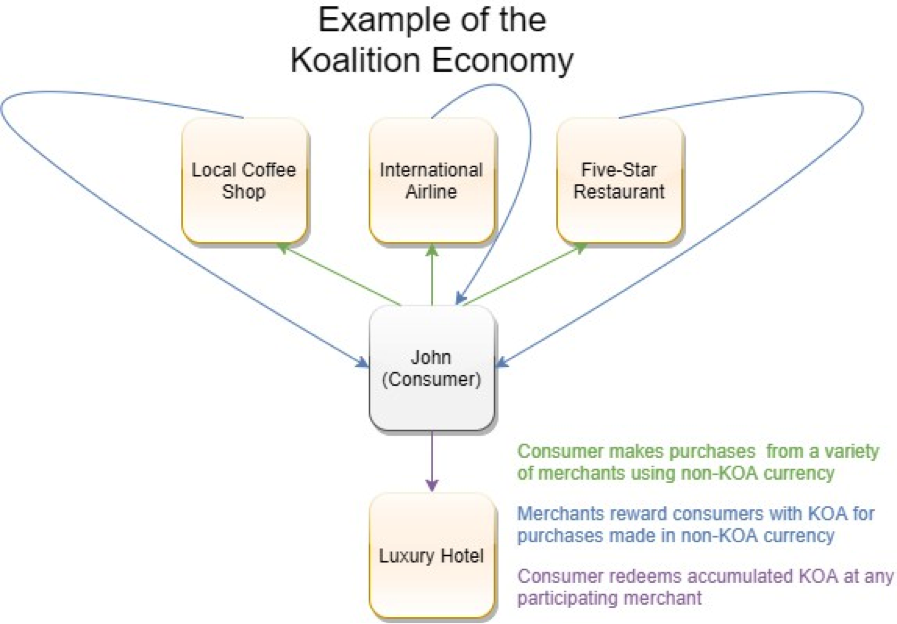
\includegraphics[keepaspectratio, width=0.7\textwidth]{images/KOAeconomy.png}
    \caption{The Koalition Economy} \label{fig:KOAeconomy}
\end{figure}

A paradigm shift in consumer behavioral and attitudinal loyalty has begun. Traditional stand-alone and coalition LPs have undoubtedly changed the dynamics of merchant competition and perpetuated the importance of relationship marketing. Koalition aims to satisfy customer demand through its vast network of merchants while maintaining integrity as a marketing tool for businesses by influencing customer buying behavior and perceptions through data analytics. Merchants now have the opportunity to embrace a disruptive technology that is bound to shake up the traditional LP economy. The following sections will discuss the intricacies of the Koalition protocol, specifically how it works, its limitations, and how it is bound to disrupt the loyalty programs space.

\subsection{Merchant Capabilities}

\subsubsection{Seamless Business Integration}
The Koalition loyalty program caters to the needs of all businesses selling products or services. From small local businesses to international corporations, each gain access to a network enhanced by blockchain technology. Small businesses gain access to a powerful marketing platform, opening their doors to a vast new customer acquisition and retention tool. Typically, small businesses do not have the infrastructure to build and support a robust LP. However, Koalition enables small businesses to integrate with current fiat payment options and will run effortlessly through autonomous contract execution. Furthermore, adopting cryptocurrencies as a means of payment eliminates large credit card transaction fees and delayed receipt of payments, which at times can be pivotal for small businesses.

For larger businesses, existing loyalty programs cannot be easily terminated from a marketing relationship perspective. Termination may be costly and negatively affect a company's image. Fundamentally, customer relationship management as a corporate strategy creates high exit barriers \cite{Rehnen16}. Therefore, Koalition offers the flexibility of two different adoption options that cater to operational risk tolerance and perceived practicality of implementation.  


\begin{enumerate}
\item \textbf{Option 1: ``Koexist" with existing LPs} \\
Merchants can choose to keep their existing LP while offering consumers the option to pay for goods and services/receive rewards in KOA or the merchant's native rewards currency. This non-invasive approach caters to businesses that have an existing LP that either wish to use both LPs indefinitely or are engineering a risk-averse exit strategy to their current LP.

\item \textbf{Option 2: Full Adoption of the Koalition Rewards Protocol} \\
Full adoption maximizes user utility for both merchants and consumers. Merchants who elect this option will replace all of the existing points in their current rewards program with KOA. The merchant must then choose how its customers who hold the native points can convert these to KOA (eg. convert cash value of native points to KOAs). Merchants who choose to fully adopt the Koalition Rewards Protocol will leverage the full extent of blockchain technology in the rewards economy. First, merchants will be fully integrated in a cooperative network where noncompetitive industries gain from each other. Second, liabilities akin to unredeemed rewards points become negligible as revenue is immediately realized.
\end{enumerate}

Streamlined onboarding of new partners perpetuates network effects. Koalition introduces an avenue for businesses of any size to partner with one another on one rewards network thus providing consumers with a convenient LP and introducing a paramount marketing opportunity to merchants. 

\subsubsection{Cross-purchasing Effects}

\textbf{Network Effects} \\
It has already been established that merchants have more to gain from a coalition LP than a stand-alone one. Liabilities are split and marketing opportunities increase as a result of LP partnerships. Koalition brings this concept to the next level with a universal LP giving merchants a superior marketing platform with virtually no liabilities (since KOA represents a real cash value) and consumers have a fungible rewards currency they can use across multiple industries. The analysis in Section \ref{sec:analysis} shows that existing merchants on the Koalition network benefit from the addition of new merchants since cross-purchasing between merchants increase. The effect here is two fold: As more consumers join the network, merchants enjoy opportunities for more data flow, customer acquisition/retention, and ultimately profits. As more merchants join the network, consumers enjoy a wider array of redemption options and purchasing power. Therefore, as the network grows, the more non-participating merchants and consumers are incentivized to join the network. 

\noindent \textbf{Equal-level Partnership and Switching Costs} \\
The Koalition loyalty program is based on an equal-level partnership model, leveraging network effects and encouraging cross-purchasing. In this model, KOA is redeemable across all merchants on the Koalition network. While it is freely redeemable between complementary merchants, a switching cost is applied between directly competing merchants. These directly competing merchants are placed in so called \textit{competition pools}. For example, consumers who accumulate points from Airline A will be unable to redeem these points from Airline B at full buying power if these two airlines are in the same competition pool. The fee percentage will be a predetermined fixed rate. Competition Pools are determined based on industry type, size of business, and operating locations. For example, two major airlines in the United States similar in market capitalization may be put in the same competition pool, but two non-chain coffee shops operating in different cities would not.
%
\begin{figure}[h] % use "t!" to force the float to start the float at top of page
    \centering
        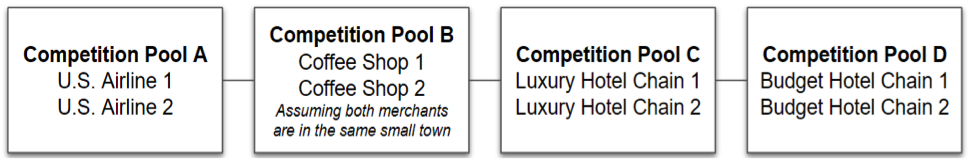
\includegraphics[keepaspectratio, width=0.7\textwidth]{images/competitionpool.png}
    \caption{Competition Pools in the Koalition Network} \label{fig:competitionpool}
\end{figure}

Furthermore, some merchants may be in the same industry, but are non-competitive amongst one another because they cater to customers in different economic backgrounds. A luxury hotel chain and a budget hotel chain would be placed in separate Competition Pools because they are not directly competitive so a consumer can have $100\%$ buying power between a luxury hotel and a budget hotel. 
%
\begin{figure}[h] % use "t!" to force the float to start the float at top of page
    \centering
        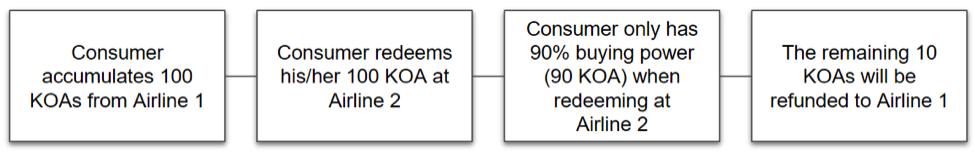
\includegraphics[keepaspectratio, width=0.7\textwidth]{images/switchingcost.png}
    \caption{Switching Costs for Consumers} \label{fig:switchingcost}
\end{figure}

Figure \ref{fig:switchingcost} above demonstrates how a consumer can use his/her KOAs that (s)he accumulates from a specific merchant. Consumers have $100\%$ buying power when redeeming KOAs at noncompetitive merchants. However, if a consumer accumulates points from one merchant and wishes to purchases a good or service from a rival merchant, then the buying power will be less. This is defined as a Switching Cost for consumers. The difference in KOA will go back to the issuing merchant. 
%
\begin{figure}[h] % use "t!" to force the float to start the float at top of page
    \centering
        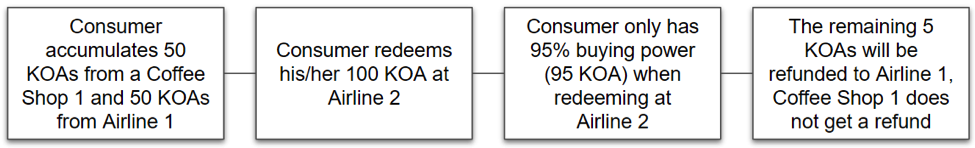
\includegraphics[keepaspectratio, width=0.7\textwidth]{images/redemption.png}
    \caption{Mixing and Matching KOA for Redemption} \label{fig:redemption}
\end{figure}

Of course, a consumer may accumulate funds from multiple purchases. Figure \ref{fig:redemption} shows a case where a consumer wishes to purchase a ticket from an airline. The consumer already has some KOA's from another competing airline as well as some KOA's from coffee shop purchases. When redeeming these points at the airline, the consumer will only pay fees with respect to the KOA's he/she accumulated from the competing airline. Koalition has injected this artificial barrier into its economy to perpetuate consumer loyalty. Though a small proportion of deadweight loss is an inevitable side-effect, competition pools and switching costs incentivize merchants to join Koalition, increasing network effects at a greater rate than if these barriers were not injected. Ultimately, an equal-level partnership scheme maximizes net utility (see Section \ref{sec:analysis}).

\subsubsection{Data Analytics for Loyalty Levers}
There are three different methods merchants use to implement their LPs:
%
\begin{enumerate}
\item \textbf{Earn-and-Burn Levers} \\ 
Customers earn rewards points through purchases from the issuing merchant. After customers accumulate enough rewards points they can ?burn? or redeem rewards points for goods and services. Frequency programs, points programs, and discount programs fall into this category.

\item \textbf{Recognition Levers} \\ 
Repeat customers receive special treatment based on how much they spend on the merchant. Travel companies and casinos popularly use this lever (eg. elite membership status).

\item \textbf{Customer Relationship Management Levers} \\ 
Targeted offers tailored to the customer are created through their purchase data. Members-only promotions and customer-specific emails are examples of CRM levers.
\end{enumerate}

Rather than rely too heavily on a particular lever, businesses must be dynamic, adapting to ever-changing markets and customer behavior. What separates successful LPs from unsuccessful ones, is how an LP combines these three approaches to optimally increase loyalty margin and incremental share \cite{Bolden14}. Koalition offers merchants real time data to enable merchants to customize their LPs. Furthermore, by analyzing customer behavior through anonymous transaction histories, Koalition can make data-driven recommendations regarding who businesses should be targeting, what scale they should operating at, where they should be focusing their resources, and when they should change their loyalty-based marketing approach. Merchants will be notified when and how they should change their LP marketing approach to balance loyalty levers and optimize profits.

\subsubsection{Increased Customer Acquisition/Retention}

\subsubsection{Leverage against OTAs}
As mentioned previously, OTAs continue to gain market share by offering flexible LPs that give customers redemption options across the travel industry.  While this type of loyalty program remains limited in scope, it caused a major disruption in a once stagnant loyalty market. Additionally, it has proven the effectiveness of offering flexible redemption options to customers. This has been problemattic for travel companies using traditional and partnership LPs due to their lack of flexibility and increased friction respectively. It has hence created a market where travel companies are stuck paying OTAs up to $20\%$ of every booking because of escalating consequences of reduced bookings from not using their services.. 

Additionally, a recent BDRC survey of US lodging loyalty members indicated that OTA loyalty programs have a $71\%$ higher proportion of millennial leisure travelers and a $44\%$ higher proportion of millennial business travelers than traditional loyalty programs \cite{}.  With millennials making up an increasing large percentage of the global consumer market and driving demand for a flexible loyalty program, businesses should be focusing on adapting to capture this market.  However, until now there has not been an easy option for companies to offer a flexible loyalty program without paying an exorbitant cost.

Koalition solves this problem by offering customers the most flexible and frictionless LP experience while eliminating booking fees for both customers and loyalty partners alike. Koalition will not offer a third-party booking service, so travel industry customers are required to book directly through the loyalty partners' native booking avenues.  Additionally, using Koalition provided data analytics, merchants can attract cost conscious customers that typically use OTAs to shop for the best rate by using the savings traditionally paid to OTAs to offer their Koalition loyalty customers personalized incentives.  These benefits will allow all Koalition Loyalty Partners the ability to provide an enhanced customer experience that exceeds the limitations of OTA LPs and provides the ultimate in customer flexibility.

\subsection{Customer Capabilities}

\subsubsection{Universal Rewards Currency}
Koalition addresses customer demand for a universal rewards currency. All merchants who join the Koalition network are partners by default. Therefore, customers are able to redeem KOA for rewards at any participating merchant or sell their KOA for market value on a cryptocurrency exchange (similar to cash back rewards programs). Since KOA is a stable coin, consumers and merchants do not have to worry about volatility risks due to holding onto the cryptocurrency and can use it similarly to a fiat currency. Transactions go beyond rewards issuance and redemption; merchants can pay merchants, consumers can pay consumers, and KOA token can also be used to make donations to charities. Buying power is constant between merchants unless the issuing merchant and redeeming merchant are in the same competition pool as previously mentioned. Furthermore, unlike traditional LP rewards points, KOA tokens never expire, so consumers can accumulate KOA for as long as they want before redemption.

\subsubsection{Frictionless Transactions}
The lack of fungibility with regards to rewards points in traditional LPs is a key frustration for customers. For example, if a consumer accumulates rewards points from one coalition LP and wants to spend them at a non-participating merchant, there may be ways to transfer points, but the process is cumbersome. Point exchange brokers like Points.com allow customers to exchange points among various merchants but charge as much as $35\%$ for the transaction. Additionally, some LPs allow consumers to redeem their points for cash value, but this action is disincentivized through unfavorable exchange rates.

Koalition provides an avenue for frictionless transactions for customers using rewards points across merchants in different industries. For merchants who incorporate the ?Koexist? or ?Full Adoption? integration methods, the friction present in traditional LPs to redeem rewards points with these merchants is removed. Since the KOA token has a consistent and stable value and doesn?t require TTPs for complex conversions during transactions, customers can easily redeem their points with any merchant that accepts KOA. This simplifies the point redemption process and gives customers more buying power because they no longer have to pay high TTP transaction costs. 

\subsubsection{Greater Redemption Opportunities}
Koalition provides the greatest flexibility in redemption options because the protocol can scale infinitely across industries. It has the potential to be redeemed anywhere, from local doughnut shops to vehicle purchases at major dealerships. Loyalty Partners choosing to accept KOA as payment for goods and services can immediately convert points to fiat currency to remove point liabilities from their balance sheets. Additionally, after the price stability protocol is implemented, Loyalty Partners and customers can hold KOA over a long period of time with limited exposure to the volatility of the cryptocurrency market.  This will allow KOA to be a frictionless loyalty currency that is optimized for transactional usage instead of acting as an investment instrument. 

Providing the greatest number of redemption options is a primary objective of Koalition and a key customer benefit. To do this, we are streamlining the Loyalty Partner integration process to ensure Koalition network growth isn?t limited by a complex onboarding process. The compounding network effect that provides increasing benefits for both customers and Loyalty Partners will fuel continued growth and greater redemption opportunities for customers.
\section{Analysis} \label{sec:analysis}
\subsection{Omnidirectional Exchange Model}
%
This section investigates the benefits of a unicurrency LP protocol. It addresses precisely how network effects form and why businesses can benefit from integrating their LPs into a protocol that promotes loyalty partnerships and increased redemption options. The following analysis combines insights from extant research to gain a comprehensive understanding of why the Koalition protocol enables a rich and interoperable LP ecosystem. Bolden \etal\ in \cite{Bolden14} argues that LPs derive their value from three inherent program characteristics: loyalty margin (LM), incremental share (IS), and program size. LM is defined as the difference between the perceived value of redeemed benefits to customers and the cost to the company for realizing those benefits. IS measures how the LP influences customer spending behavior-- it is the difference between total customer expenditure after the introduction of a LP and total customer expenditure beforehand. Lastly, program size is the share of the businesses' revenue generated from the LP. Goel's work in \cite{Goel17} introduces the notion of merchant utility and social welfare in coalition LPs. Using a bilateral negotiation model, Goel provides insight on how companies can optimally set their exchange rates with respect to these measures. In order to develop a unicurrency LP protocol, it is necessary adopt a model which eliminates exchange rates and accounts for the incremental utility of additional merchants to existing partners. %but preserve the original definitions of utility and social welfare. 

To develop this model, it is important to understand how two merchants benefit from a joint program. In this scenario, merchant $i$ and merchant $j$ have a loyalty partnership where type-$j$ customers (merchant $j$'s loyal customers) wish to avail services from merchant $i$-- type-$j$ customers are more likely to visit merchant $i$ if they are able to collect points at $i$ to redeem at merchant $j$. This excess demand is beneficial for merchant $i$ because it brings in immediate revenue from type-$j$ customers as well as future revenue from these new customers who may prefer merchant $i$ over its competitors in the future. Merchant $i$ also gains immediate revenue from type-$i$ customers redeeming points at merchant $i$, collected from merchant $j$. This is because merchant $i$ receives immediate revenue from the points redeemed since these points have market value. Merchant $i$ also continues to obtain immediate revenue from type-$i$ customers who collect and redeem points at merchant $i$ as if it were a stand-alone LP. On the other hand, every type-$i$ customer visit to merchant $j$ may result in a loss of immediate/future revenue to merchant $i$. This loss is greater with a more competitive merchant $j$, but is negligible if merchant $j$ provides a complimentary service. Lastly, merchant $i$ incurs a redemption cost for every point redeemed by type-$i$ and type-$j$ customers.
%
\begin{figure}[H] % use "t!" to force the float to start the float at top of page
	\centering
	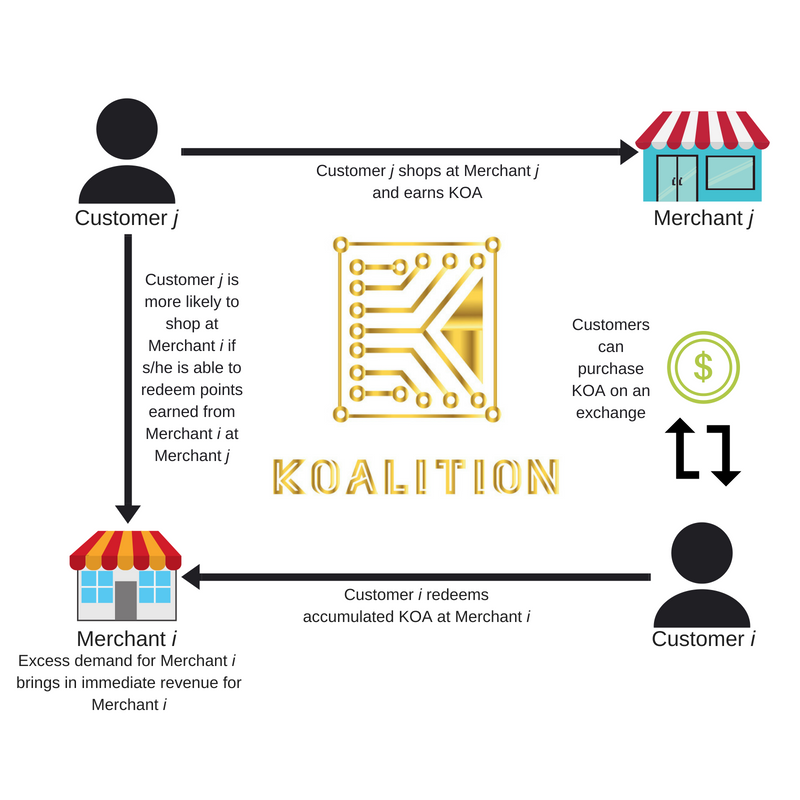
\includegraphics[keepaspectratio, width=0.5\textwidth]{images/PointRedemption.png}
	\caption{Point Redemption} \label{fig:PointRedemption}
\end{figure}

First, define $\theta_{ij}$ as the rate of type-$i$ customers collecting points at merchant $j$ with the intention of redeeming them at merchant $i$. Next, $c_{ij} \in [0, 1]$ is a measure of the competitiveness between merchant $i$ and $j$ and is symmetric, \ie\ $c_{ij} = c_{ji}$. Next, the customer acquisition value, $a_i \geq 0$, represents the value the merchant obtains per point earned and converted by a type-$j$ customer. Again, this can be interpreted as the combination of immediate and future revenue from type-$j$ customers. Lastly, $q_i$ is defined as the difference between the market value per point redeemed and the cost to the merchant per point redeemed. Note that the market value per point redeemed is equivalent to the customer's perceived value per point, which makes $q_i$ exactly equivalent to the LM, as defined earlier. 

Given the above, the two-merchant utility for $i$ is
%
\begin{align*}
u_i = \theta_{ii}q_i + \pi_{ij}
\end{align*}
%
where $\pi_{ij}$ represents the incremental utility gained from merchant $i$ and $j$ establishing a loyalty partnership and is defined as
\begin{align*}
\pi_{ij} = \theta_{ji}a_i - \theta_{ij}(a_j c_{ij} - q_i)
\end{align*}
%
\textit{Social welfare} (\ie\ sum of incremental utilities) between merchants $i$ and $j$ is defined as
\begin{align*}
\pi_{ij} + \pi_{ji} = \theta_{ij}(a_j(1-c_{ij}) + q_i) + \theta_{ji}(a_i(1-c_{ji}) + q_j)
\end{align*}
Notice that social welfare is maximized when $c_{ij} = c_{ji} = 0$. Thus, It seems that loyalty partnerships that are the most beneficial are between two merchants that provide complementary services. All else equal, as the two merchants become more competitive (\ie, $c_{ij} > 0$), social welfare decreases. While social welfare decreases with increased competition, an environment where merchants offer substitutable services may cause type-$j$ customers to become type-$i$ customers (and vice versa). This is reflected as an increase in $\theta_{ii}$ (or $\theta_{jj}$) and so while social welfare decreases, individual utility, $u_i$ ($u_j$), may increase at the cost of merchant $j$ (merchant $i$). 

For the general case, the $N$-merchant utility for $i$ is
\begin{align*}
u_i = \theta_{ii}q_i + \Pi_i
\end{align*}
%
where $\Pi_i$ is the \textit{incremental network utility} and is defined as
\begin{align*}
\Pi_i & = \pi_{i1} + \pi_{i2} + \pi_{i3} + ... + \pi_{i(N-1)} + \pi_{iN} \\
& = \sum_{k=1}^N \big[\theta_{ki}a_i - \theta_{ik}(a_k c_{ik} - q_i) \big]
\end{align*}
%
Note that as $q_i$ (LM) increases, individual and incremental network utility increase. The general form of social welfare for $N$-merchants follows from the above definitions and is defined below. Note that the effect of non-competition for the two-merchant case generalizes to the $N$-merchant case, \ie\ $c_{ik} = 0$ for all $i, k \in \{1,...,N\}$ and $i \neq k$ maximizes social welfare. 
\begin{align*}
\Pi_1+ \Pi_2 + ... + \Pi_{N-1} + \Pi_N = \sum_{i=1}^N \sum_{k=1}^N \big[\theta_{ki}a_i - \theta_{ik}(a_k c_{ik} - q_i) \big]
\end{align*}
%
Furthermore, in the special case where all merchants provide complimentary services, $\Pi_i > 0$ for all $i \in \{1,...,N\}$ assuming $\sum_{k=1}^N\theta_{ki}$ and  $\sum_{k=1}^N\theta_{ik}$ are strictly positive and $q_i$ is non-negative. In other words, if competition between LPs is negligible in a protocol that permits customers to easily exchange their points among individual LPs with positive LMs, then merchants who join the protocol benefit because they gain additional customers. Also, since incremental network utility is positive for any given merchant, then as the number of merchants increases, social welfare also increases.

Next, we account for competition and determine under what LMs social welfare increases as the number of loyalty partnerships in the protocol grows. In order for social welfare to grow as $N$ grows, each additional merchant must have positive incremental network utility ($\ie\ \Pi_i > 0, \forall i \in \{1,...,N\}$). 
%
\footnote{Better to put condition in terms of LM?-- Need to find out: Do customers spend more money with more members in a coalition (this affect $a_i$)? Do they become more frequent visitors at any given merchant in a coalition? (this affects $\theta_{ij}$) Do they gain more "new" customers as coalition increases? (this affect $a_i$). Note lower $a_i$ is easier to obtain than a higher one since this means lower req'd change in customer behavior}
%
To achieve this condition, the LM ($q_i$) of any merchant $i$ must satisfy the following inequality:
\begin{align*}
q_i > \frac{\sum_{k=1}^N \theta_{ik} a_k c_{ik} - a_i \sum_{k=1}^N \theta_{ki}}{\sum_{k=1}^N \theta_{ik}}
\end{align*}
%
The first term of the numerator on right-hand side of the inequality is the \textit{total perceived cost of competition} to merchant $i$. The second term is the product of the total collection ratio and the customer acquisition value of merchant $i$, which is defined as the \textit{customer acquisition volume}.\footnote{come up with a more intuitive explanation of what this is and a good name that captures this product}

As the total perceived cost of competition to $i$ increases, merchant $i$'s LM must also increase to maintain positive incremental network utility (\ie\ continue to individually benefit from the network). This increased cost to merchant $i$ results from merchants on the protocol who offer substitutable services (increase $c_{ik}$) and are able to generate more immediate/future revenue merchant $i$'s loyal customers (increased $a_{k}$). One way to offset this increased cost from competition is to introduce \textit{switching costs} between competitive merchants. This serves as a barrier to discourage customers from availing services from a competitor and its effect can be interpreted as a decrease in $c_{ik}$. In the face of competition, switching cost can help merchants maintain a smaller LM but still achieve positive incremental network utility.  Lastly, for the special case of non-competitive merchants, the non-negativity assumption on $q_i$ (LM) can be relaxed. As long as the LM is greater than the negative of the customer acquisition volume, merchant $i$ is guaranteed to have positive incremental network utility. Note that this does not guarantee positive merchant utility (\ie\ $u_i > 0$) as the magnitude of the stand-alone LP utility may be greater than incremental network utility. Hence, while a merchant with a negative LM may still contribute to social welfare, it does not guarantee positive individual utility. 

On the other hand, as customer acquisition volume increases, the required LM to benefit on the network will decrease. This increase in volume can result from two things happening: 1) more ``new customers" collect points at merchant $i$ than customers leaving $i$ to collect from other merchants and 2) customers expend more at merchant $i$. This increase can essentially be attributed to an increase in the IS of a merchant's LP, hence it is necessary to show that as the number of merchants, $N$, increases, the LP's IS also increases (\ie\ the growth of the LP protocol leads to increased customer activity and spending). 

\subsection{Koalition LP Network}
%
According to \cite{Breu15}, there are two primary types of coalition LPs: \textit{dominant LP model} and \textit{equal-level partnership model}. In the former model, the dominant business runs the LP therefore communication and marketing revolves around the offerings of the dominant LP and is augmented by the offerings from the other partners. In the latter model, the coalition LP is typically run by a TTP specializing in LP management. Marketing efforts and communication towards customers are done through joint redemption promotions and increased redemption options. Using the omniexchange model developed in the last section, this section compares the \textit{utility} of these two types of coalition LP designs on the Koalition protocol. Specifically, it is shown that if individual merchant LPs can achieve a high enough LM, the equal-level partnership model promotes greater individual utility and social welfare compared to the dominant LP model. Furthermore, this section introduces the notion of switching costs in the form of fees when redeeming points between two directly competing firms. For example, in order to redeem points that originated from American Airlines at United Airlines, the customer must pay a redemption fee. It is found that by carefully selecting the switching cost, the Koalition protocol is able to leverage the utility of firms with smaller LMs. 
%
\begin{figure}[h]
	\centering
	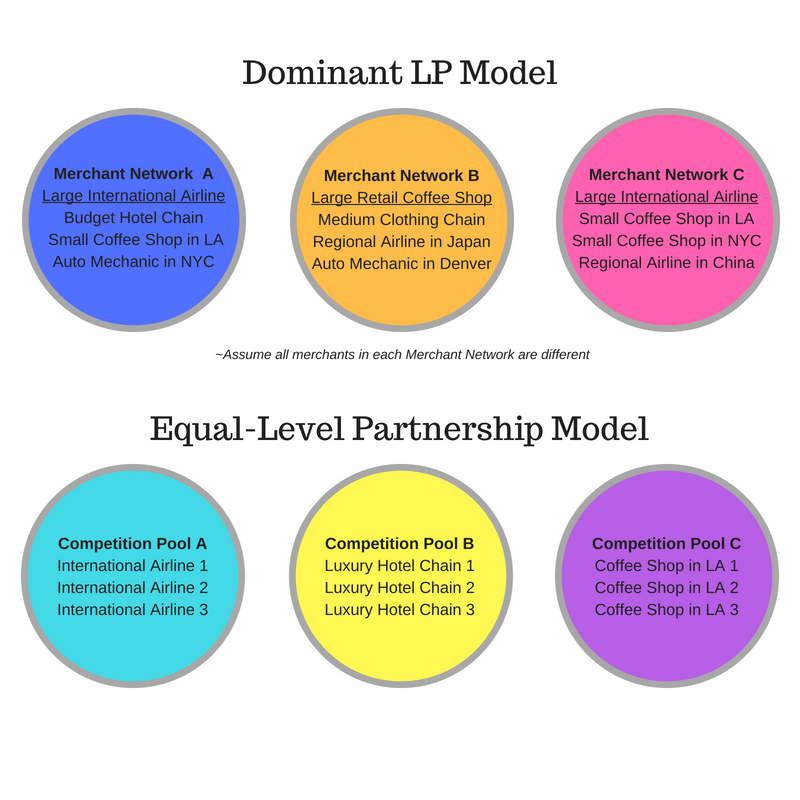
\includegraphics[keepaspectratio, width=0.7\textwidth]{images/DomEqual}
	\caption{Dominant LP Model vs Equal-Level Partnership} \label{fig:DomEqual}
\end{figure}

First, the implementation of a dominant LP type model in the Koalition protocol is investigated. Imagine a unicurrency LP protocol where the set of all merchants is defined as $M \subseteq \mathbb{Z}_{\geq 0}$ and  
groups of complimentary merchants $N_k$ form. Specifically, $N_k$ is defined as the $k$-th network group where merchants $i$ and $j$ and belong to $N_k$ in the sense that $i$, $j \in N_k$ and $i \neq j$. A merchant $i$ joins a network group such that $c_{ij} = c_{ji} = 0$ or $c_{ij} << 1$ for all $j \in N_k$. In other words, merchants will prioritize groups that minimize their competition to every other merchant in the group. Furthermore, denote $<N_k>_{k \in \{1,...,m\}}$ to be a partition of $M$, where $m$ represents the number of coalition groups formed on the protocol. In this scheme, customers normally belong to a specific network group and are able to redeem and collect points freely in that group. Customers are also free to collect and accumulate points at different network groups (similar to how customers now can collect and accumulate points from different LPs). On the other hand, while customers have the option to redeem their points at a different network group, these redemptions will be subject to switching cost. \textbf{image of what this looks like?}

In an equal-level partnership type model on the Koalition protocol, customers are free to exchange points across the protocol without the artificial barriers raised by network groups. Instead of having to pay switching costs to avail services from merchants in different groups (who may even provide complimentary services), one only has to pay a fee when redeeming points at merchants who are direct competitors. \textbf{image here?} This scheme gives customers more redemption options, better leverages network effects, and promotes inclusion. Intuitively, these benefits result in higher network utility and increased social welfare (compared to the dominant LP model). First, let us define the network utility of a merchant $i$ in the equal-level partnership model follows:
%
\begin{align*}
\Pi_i^* & = \sum_{k \in M} \big[\theta_{ki}a_i - \theta_{ik}(a_k c_{ik} - q_i) \big]
\end{align*}
%
For simplicity, there is a slight abuse in notation with $M$ and $N_k$ as they are still the sets defined above, minus the subject merchant (in this case merchant $i$).  Next, the network utility of some merchant $i$ belonging to network group $N_\ell$ in the dominant LP model is defined as follows:
%
\begin{align*}
\Pi_i & = \sum_{k \in N_\ell} \big[\theta_{ki}a_i - \theta_{ik}(a_k c_{ik} - q_i) \big] + \sum_{j \in M - N_\ell} \big[\epsilon \theta_{ji}a_i - \epsilon \theta_{ij}(a_j  c_{ij} - q_i) \big]
\end{align*}
%
Note the introduction of the $\epsilon$ in the second term of the dominant LP network utility equation. Switching cost is encoded in the equation through $\epsilon \in (0,1)$, signifying a decrease in collection rates-- as $\epsilon$ decreases, switching cost increases (and vice versa) hence the rate at which customer collect points at merchant $i$ and merchants other than $i$ also decreases. 

The goal is to prove that individual utility is higher in the equal-level partnership design (\ie\ $\Pi_i^* > \Pi_i$ for all $i \in M$) and that social welfare is also higher in the equal-level partnership design. Theorem \ref{thm:utility} in the appendix shows that merchants benefit more in an equal-level partnership LP model than in a dominant LP model. Even when switching costs exists between directly competing merchants in the equal-level partnership model, these merchants benefit from greater cross-purchasing compared to merchants in the dominant LP model. This is because in the latter model, complementary merchants are grouped in different networks leading, reducing the collection rate between them. In the equal-level partnership model, collection rates between merchants are higher since switching cost are limited to only directly competing merchants across the whole protocol. Furthermore, note only do merchants individually benefit more in an equal-level partnership LP model, Corollary \ref{thm:welfare} shows that all merchants are better off in this model compared to a dominant LP model. Intuitively, if cross-purchasing between merchants is higher in the former model than in the latter model, then these merchants benefit more as a whole. Hence social welfare of merchants in the equal-level partnership model is greater than in the dominant LP model.

The cross-purchasing phenomenon of equal-level partnership models is well known in the literature (see \cite{Dorotic12}), but is difficult to implement at a large scale due to integration barriers imposed on potentially new partners (discussed in Section \ref{sec:BCloyalty}). A blockchain solution would remove these barriers allowing coalitions based on equal-level partnership models to naturally form and thrive. Thus, the Koalition protocol will be based off the equal-level partnership model, enabling a rich and interoperable LP environment that minimizes friction, promotes the creation of loyalty partnerships, and improves overall customer experience. 

\subsection{KOA Treasury}
Koalition utilizes a non-collateralized stabilization scheme that keeps KOA price volatility low, making it a practical and frictionless medium of exchange. The KOA treasury is a smart contract that functions like a central bank in that it maintains an elastic supply of distributed KOA and keeps the coin at a fixed USD target price range. The target price range is defined as the range of prices that fall (inclusively) between $\delta^+$ above $p^*$ and $\delta^-$ below $p^*$, where $p^*$ is a \textit{baseline target price}, $\delta^+$ is the \textit{upper threshold rate}, and $\delta^-$ is the \textit{bottom threshold rate}. In other words, the target price range is any price that does not exceed $\delta^+$ percent of the baseline price or is $\delta^-$ percent lower.

In a bull market when the price of KOA exceeds $\delta^+$ percent of the baseline, the KOA treasury initiates an auction tranche. During an auction tranche, the treasury mints and auctions out new KOA by an amount proportional to the increase in price. The price at which the treasury auctions out KOA is strictly lower than its market price by $\alpha^+$ (\textit{upper arbitrage rate}), pulling demand off of exchanges and creating downward pressure on the market price. The seigniorage gained from the auction tranche is stored in the seigniorage pool.
%
In a bear market when the price of KOA declines to $\delta^-$ percent below the baseline, the KOA treasury initiates an absorb tranche. During this period, the treasury buys back  KOA at price strictly higher than market price by $\alpha^-$ (\textit{bottom arbitrage rate}) in an effort to pull supply off of the exchanges and create an upward pressure on the market price. If the capital in the seigniorage pool is insufficient to stabilize a continuous decline in price, the treasury will issue bonds entitling users willing to redeem their KOA at a discounted price during future auction tranches. Figure \ref{fig:treasury} displays a high level overview of the KOA treasury and its discussed features.

One of the primary challenges of this type of stabilization scheme is that it is difficult to analyze the safety margin of the seigniorage pool. How much seigniorage must the pool contain such that it will never be depleted? If that is impractical, how much seigniorage must the pool contain such that the probability of running out of seigniorage is small? Under what market conditions will this hold? What should the baseline price be set to? What values should the threshold and arbitrage rates be set to? Some of the analysis required to answer these questions are discussed in the next section.
%
\begin{figure}[] % use "t!" to force the float to start the float at top of page
    \centering
        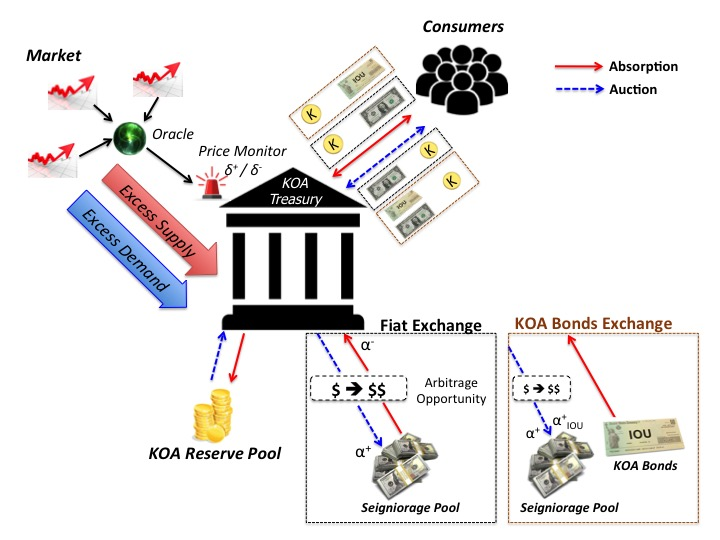
\includegraphics[keepaspectratio, width=0.7\textwidth]{images/treasury.jpg}
    \caption{High Level Overview of the KOA Treasury} \label{fig:treasury}
\end{figure}

\subsubsection{Price and Treasury Dynamics}
The price of KOA is assumed to evolve as a \textit{random walk} when within the target price range and jumps back to the baseline price during tranche periods, as follows
%
\begin{equation} \label{eq:price}
\begin{aligned}
p_{t+1} =
\begin{cases}
      p_t + \xi_t, & p_t \in [p^* - \delta^- p^*, p^* + \delta^+ p^*] \\
      p^*, & \text{otherwise}
\end{cases}
\end{aligned}
\end{equation}
%
where $t \in \{0,...,T\}$ and the $i$-th tranche occurs at time $t_i$. The sequence $\{\xi_t\}$ is \textit{independent} and \textit{identically distributed} (\iid), \ie\ $\xi_t$ $\sim$ \iid\ $(\mu, \sigma^2)$. In order to make this assumption, it is sufficient to pick values of $t$ at which to observe the market price such that price evolutions lack non-randomness and follow the efficient market hypothesis (EMH). Proving EMH justifies the random walk model in Equation \ref{eq:price}. It was found that 1 day price observations of Bitcoin showed a lack of significant non-randomness \textbf{(solver world or just prove this ourselves)}, which is further validated by a study done in \cite{Bartos15}. Hence, the oracle in Figure \ref{fig:treasury} will observe the price of KOA at 1 day intervals. This price measurement will be taken as the average price of the price reported from various market trackers.

In order to analyze the robustness of the KOA treasury, the effects of tranches on the distributed KOA supply, the KOA reserve, and the Seigniorage pool are modeled as follows,
%
\begin{align*}
& \qquad \quad \, Q_{i+1} = Q_i + u_i \\
& \qquad \quad \, R_{i+1} = R_i - u_i \\
& u_i =
\begin{cases}
      Q_i \delta^+,  & p_i = (1+\delta^+)p^* \\
      -Q_i \delta^-,  & p_i = (1-\delta^-)p^*
\end{cases}  \\
S_{i+1} = & \begin{cases}
      S_i + p^*(1+\delta^+)(1-\alpha^+)u_i, & u_i > 0 \\
      S_i - p^*(1 - \delta^-)(1+\alpha^-)u_i, & u_i < 0
\end{cases} 
\end{align*}
%
where $i \in \mathbb{Z}_{>0}$ represent an index for the tranche occurrences during some time period $T$, $Q_i$ represents the supply of KOA in distribution, $R_i$ the balance of KOA in the treasury reserves, and $S_i$ the total amount of fiat in the seigniorage pool during the $i$-th tranche. Also, $u_i$ represents the amount of KOA the treasury auctions or absorbs during the $i$-th tranche where $p_i$ is the price of KOA during the $i$-th tranche. Note that there are several assumptions made in this model. First, it assumes that a $\delta^+$ (or $\delta^-$) change in price will require a $\delta^+$ (or $\delta^-$) change in KOA supply distributed in order to bring the price back to $p^*$. Secondly, the price goes back to baseline instantaneously once the treasury distributed (or absorbs) the required KOA. \textbf{illustration of indexing here}

Now a tranche is initiated whenever the price of KOA ``walks out" of the target price range, increasing or absorbing the supply as required to reconnect to $p^*$. The sequence of \textit{waiting times} $\{ \tau^+_i \}_{i \geq 1}$ that the price, $p_t$, falls above the upper threshold price rate is assumed to be a sequence of independent exponential random variables with mean $\lambda^+$ (termed the \textit{auction rate}). Let $T_n = \sum_{i=0}^n \tau_i^+$  be a random variable that represents the time the price exceeds the upper threshold for the $n$-th time. The number of times the price exceeds $\delta^+$ percent of $p^*$,
%
\begin{equation} \label{eq:bullcount}
N_t = \sum_{n \geq 1} 1_{t \geq T_n} 
\end{equation}
%
is a Poisson process with probability distribution $\mathbb{P}(N_t = n) = e^{-\lambda^+ t} \frac{(\lambda^+ t)^n}{n!}$. The sequence of waiting times $\{ \tau^-_i \}_{i \geq 1}$ that $p_t$ falls below the bottom threshold price rate has similar characteristics but with mean $\lambda^-$ (called the \textit{absorb rate}). The definition of $T_m$ is similar to that of $T_n$, except that it is the time the price drops below the bottom threshold for the $m$-th time. Hence, the number of times the price declines below $\delta^-$ percent of $p^*$ is defined as follows
%
\begin{equation} \label{eq:bearcount}
M_t = \sum_{m \geq 1} 1_{t \geq T_m} 
\end{equation}

\subsubsection{Absorption Tranche}
\jacomment{Now that the treasury is fully characterized, it is now possible to answer the first of the questions posed earlier: how much seigniorage must the pool contain such that it will never be depleted? Given that $R_0$ is chosen to be sufficiently large}{Maybe add $S_{M_t}$ explanation here?} \jkcomment{This is a test}{another test}]%
%
\footnote{In fact it was discovered in \cite{Ath08} that buffer stock reserves containing a small percentage of the distributed equilibrium supply was sufficient in maintaining price stability. In other words, if the supply is close to the fundamental value (FV) supply, a reserve supply of about $1$-$2$ percent of the FV supply will be able to keep price stable. Setting $R_0$ such that $R_0 >> S_0$, should satisfy this condition as the reserve has more than it needs to allow the initial supply to get to the FV supply and maintain the supply there without running out.} 
%
and that there is not a complete loss in demand, this question can be answered by considering a scenario where prices are monotonically decreasing over some period during T (\ie\ $p_{t+1} \leq p_t \leq ... \leq p_0$). In this situation, the treasury initiates a series of absorption tranches that absorbs a maximum seigniorage amount of $S^*$. 
%
\begin{equation} \label{eq:Smax}
S^* = p^*(1-\delta^-)(1+\alpha^-)Q_0
\end{equation}
%
This is defined as the \textit{Optimal Seigniorage} and follows from Lemma \ref{lemma:Smax} in the appendix.

In other words, the KOA treasury will never deplete its seigniorage pool if it contains at or above $S^*$ prior to a worst case scenario bear market. The problem is that this amount can be fairly large and grows as the distributed KOA supply grows. Collecting the required capital to meet this amount may be impractical and as the seigniorage pool grows, this stabilization scheme runs into similar problems that plague non-collateralized schemes. Hence, it is highly desirable to have a small and efficient, but robust seigniorage pool that will be able to handle a large band of worst-case market scenarios. A treasury that meets this criteria is defined as one with a \textit{Robust-and-Agile} (\textit{RAA}) seigniorage pool. Hence, the next task is to answer the second question posed above: how much seigniorage must the pool contain such that the probability of running out of seigniorage is small?

A \textit{RAA} seigniorage pool, $\hat{S} = \epsilon S^*$ where $\epsilon \in \mathbb{R}_{>0}$ is called the \textit{RAA parameter}, is one that has a lower than 30\% chance of being depleted during some period $T$. Theorem \ref{thm:bearbounds} in the appendix shows that the probability of depleting the treasury during this time is defined as follows.
%
\begin{equation} \label{eq:bearbounds}
\begin{aligned}
& 1 - \Phi (\sign(\log_{1- \delta^-}(1-\epsilon) - \lambda^- +1) \sqrt{(2H(\lambda^-, \log_{1- \delta^-}(1-\epsilon) +1))}) \\
& < \prob(\text{deplete}) \\
& < 1 - \Phi (\sign(\log_{1- \delta^-}(1-\epsilon) - \lambda^-) \sqrt{(2H(\lambda^-, \log_{1- \delta^-}(1-\epsilon)))})
\end{aligned}
\end{equation}
%
where $\sign(\cdot)$ is the signum function and $\Phi(\cdot)$ is the standard normal cumulative distribution function. Given any $S_0$ (as defined by being some $\epsilon$ percent of $S^*$), the probability that it will be depleted during period $T$ can be easily computed by Equation \ref{eq:bearbounds}. Per the definition of a RAA seigniorage pool, $\hat{S}$ is defined as any $\hat{S} = \epsilon S^*$ such that $\prob(M_T \geq  \log_{1- \delta^-}(1-\epsilon)) <$ 0.3.

\subsubsection{Auction Tranche}
Now that the amount of seigniorage required to handle a band of bearish behavior has been determined, the next step is to determine the bull market bull behavior required to replenish the pool and ensure the required seigniorage exists at the beginning of period $T+1$. Consider a scenario where price is monotonically increasing after a bear market and the number of times the price exceeds $\delta^-$ takes on the counting Poisson Process in Equation \ref{eq:bullcount}. The treasury therefore initiates a series of auction tranches causing the seigniorage pool to replenish incrementally as follows.
%
\begin{align*}
\Delta S_i^+ = S_{i+1}^+ - S_i^+ = p^*(1+\delta^+)(1-\alpha^+)u_i 
\end{align*}
%
Again, since $u_i = Q_i\delta^+$ and $\Delta S_i^+ = p^*(1+\delta^+)(1-\alpha^+)Q_0(1-\delta^+)^i\delta^-$ follows, then $S_{N_t}$ denotes the amount of reserves auctioned off during some time $t$ and is defined as
%
\begin{equation} \label{eq:Sreplenish}
S_{N_T} = p^*(1+\delta^+)(1-\alpha^+)Q_0\big((1+\delta^+)^{N_T} - 1 \big)
\end{equation}
%
The objective is to determine the probability that the seigniorage pool will be replenished by a bull market during $T$, \ie\ $\prob(S_{N_T} \geq S_{M_T})$. In order to carry out the analysis, the following \textit{sufficiency assumptions} are made
%
\begin{equation*} \label{eq:sufficientassumptions}
\delta^+ \geq \alpha^-, \quad \delta^- \geq \alpha^+
\end{equation*}
%
These assumptions ensure that $N_T \geq M_T$ is a \textit{sufficient} condition for the $S_{N_T} \geq S_{M_T}$ inequality to hold. Thus, since $N_T \geq M_T$ implies this original inequality, then $\prob(S_{N_T} \geq S_{M_T})$ can be closely approximated by $\prob(N_T \geq M_T)$.

Since $N_T \sim$ Poiss($\lambda^+$) and $M_T \sim$ Poiss($\lambda^-$), where $N_T$ and $M_T$ are independent RVs, $W_T = N_T - M_T$ takes on a \textit{Skellam distribution}, in other words $W_T \sim$ Skellam($\lambda^+ - \lambda^-$, $\lambda^+ + \lambda^-$). The probability of replenishing the treasury can be computed easily as follows
%
\begin{equation} \label{eq:bullbounds}
\prob(\text{replenish}) = \prob(W_T \geq 0) = 1 - \psi(0, \lambda^+, \lambda^-)
\end{equation}
%
where $\prob(\text{replenish}) = \prob(N_T \geq M_T)$ and $\psi(\cdot)$ is the CDF of $W_T$, which has no closed form solution but can easily be numerically computed. The analysis above was conducted for a worst-case  scenario in which the price decreases continuously, but the result applies to the more general case where the price changes non-uniformly throughout some period $T$. 

\subsection{Data and Discussion}

\subsubsection{Finding Auction and Absorb Rates} \label{thresholdDiscussion}
In order to compute the bounds, it is necessary to know the values for $\lambda^+$ and $\lambda^-$. These rates represent the number of times the price exceeds $\delta^+$ or declines below $\delta^-$ of the target price, respectively, in a given period of time. Table \ref{table:avgdata} shows different values of $\lambda^+$ and $\lambda^-$ for various cryptocurrencies at different values of $\delta^+$ or $\delta^-$ between November 1, 2017 to April 1, 2018 (\ie\ $T = 5$ months). During the earlier stages of this period, the cryptocurrency market experienced a large surge in market cap as it thrusted into the media spotlight. Holidays, increasing regulations in Asia, and overvaluation in the earlier months resulted in a steady decrease in price in the latter months of this period. It is possible to observe worst-case volatility behavior by measuring $\lambda^+$ and $\lambda^-$ during periods of high speculation, allowing Equations \ref{eq:bearbounds} and \ref{eq:bullbounds} to yield conservative estimates. Furthermore, these observed values are likely higher than they would be if a price stabilization scheme were in place for each cryptocurrency. Hypothetically, if the market knew the price of a cryptocurrency would be stabilized endogenously, then speculation should be significantly less and price changes should result from changes in true demand. 
% Notes to add throughout
%When determining $\lambda^+$ and $\lambda^-$, it is assumed that the price at each time $t$ (see Equation \ref{eq:price}) is \textit{independent} of the price at any other time and that the bear periods are \textit{independent} of the bull periods (\ie\ $M_t$ is independent of $N_t$). 
%For the first assumption, it is sufficient to pick values of $t$ at which to observe the market price such that a random walk model if valid. It was found that 1 day price observations of Bitcoin showed a lack of significant non-randomness {solver world or just prove this ourselves}, which was further validated by studies {cite "does bitcoin follow hypothesis of efficient market"}. 
%Reference "Price stabilization via Buffer stocks" to justify 100 billion coin supply. Only a fraction of equilibrium supply capacity is required in reserves to stabilize price.

Table \ref{table:avgdata} highlights the relationship between the set threshold rates and their respective absorb and auction rates. It can be seen that for all cases, as the price threshold rates increase the treasury intervenes less to stabilize the price. This is expected since a larger target price range allows the price to evolve and possibly self correct on its own. Thus, Equations \ref{eq:Sdeplete} and \ref{eq:Smax} show that the treasury requires less seigniorage in order to stabilize back to the target price at higher values of $\delta^-$. This is consistent with a finding on exchange rate stabilization using buffer stocks in \cite{Kot08}, in which central banks incur less cost when they attempt to track the exchange rate towards the currency's fundamental value. Similarly, if the target price range increases it will more likely contain KOA's fundamental value ($\tilde{p}$), requiring less intervention from the treasury. The value of $\delta^-$ must be high enough to increase the likelihood of this condition, but not too high where significant amounts of volatility is tolerated. This value will also depend on how far $p^*$ is from KOA's fundamental value (which will depend on the true demand of KOA). The further $p^*$ is from $\tilde{p}$, the greater $\delta^-$ must be in order to maintain the likelihood of $\tilde{p}$ in the target price range. On the other hand, the upper threshold rate can be set to a relatively low value to keep the price close to the target price, while accumulating more seigniorage. How the threshold rates are adjusted and at what value to set $p^*$ will be discussed in a later section. %Talk about this further in the next section
%
\begin{table}[]
\centering
\begin{tabular}{|c|c|c|c|c|c|c|}
\hline
\multicolumn{1}{|l|}{}                                               & \multicolumn{3}{c|}{$\lambda^+$}          & \multicolumn{3}{c|}{$\lambda^-$}       \\ \hline
\multicolumn{1}{|l|}{}                                               & $\delta^+=0.15$  & $\delta^+=0.20$ & $\delta^+=0.30$            & $\delta^-=0.15$  & $\delta^-=0.20$ & $\delta^-=0.30$ \\ \hline
Bitcoin                                                          & $12$ & $8$ & $6$           & $9$  & $6$ & $3$     \\ \hline
Ethereum                                                        & $11$    & $8$    & $5$             & $9$ & $6$ & $3$     \\ \hline
\begin{tabular}[c]{@{}c@{}}Ripple\end{tabular} & $14$    & $13$    & $8$ & $13$        & $10$        & $4$     \\ \hline
\begin{tabular}[c]{@{}c@{}}OmiseGo\end{tabular} & $17$    & $11$    & $6$ & $13$        & $7$        & $3$     \\ \hline
\end{tabular}
\caption{Values of $\lambda^+$ and $\lambda^-$ for Various Cryptocurrencies During a $T = 5$ month period} \label{table:avgdata}
\end{table}

\subsubsection{Robustness of KOA Treasury}

This section discusses the robustness of the KOA treasury and how it is affected by the treasury parameters. Combining the complement of Equation \ref{eq:bearbounds} with \ref{eq:bullbounds} yields bounds on the probability that the treasury will maintain its seigniorage pool during a given period. This is called the treasury's \textit{robustness probability} and is shown below
%
\begin{equation} \label{eq:robustbounds}
\begin{aligned}
& (1-\psi(0, \lambda^+, \lambda^-)) \prob^-(S_{M_T} \geq S_0) \\
& < \prob(\text{robust}) \\
& < (1-\psi(0, \lambda^+, \lambda^-)) \prob^+(S_{M_T} \geq S_0)
\end{aligned}
\end{equation}
%
where $\prob^-(S_{M_t} \geq S_0) = \Phi (\sign(\log_{1- \delta^-}(1-\epsilon) - \lambda^-) \sqrt{(2H(\lambda^-, \log_{1- \delta^-}(1-\epsilon)))})$, $\prob^+(S_{M_t} \geq S_0) = \Phi (\sign(\log_{1- \delta^-}(1-\epsilon) - \lambda^- +1) \sqrt{(2H(\lambda^-, \log_{1- \delta^-}(1-\epsilon) +1))})$, and $\prob(robust) = \prob(S_0 \geq S_{M_T} \cap N_T \geq M_T)$. Note that these bounds depend highly on the treasury's parameters at each period. 

Consider when the treasury maintains a seigniorage pool greater than $S^*$ (\ie\ $S_0 \geq S^*$)-- in this case the treasury has no chance of depleting its seigniorage pool in a given period. The treasury's robustness probability will depend only on its replenish probability, which is the probability that there is greater overall demand in that period (probability of more auctions than absorptions). The threshold rates $\delta^+$ and $\delta^-$ significantly impact this probability due to their relationship with $\lambda^+$ and $\lambda^-$, respectively (see Section \ref{thresholdDiscussion}). The threshold rates should be chosen not only to control a range of volatility, but also so that $\lambda^+ >> \lambda$. It is sufficient to say that values for $\lambda^+$ and $\lambda^-$ such that $\lambda^+ \geq 2 \lambda^-$ meets this condition. In the case where $S_0 \geq S^*$, the robustness of the treasury will depend strictly on the relative values of $\lambda^+$ and $\lambda^-$. Fortunately, due to the cryptocurrency market's (super)-exponential growth in market capitalization (and demand) \cite{ElBahrawy17}, it is expected that $\lambda^+ >> \lambda^-$ for a given $\delta^+$ and $\delta^-$ for $\delta^+ \leq \delta^-$. Hence, the rate at which the KOA treasury collects seigniorage will be greater than the rate that it spends them. Considerations for choosing the threshold rates are discussed further in Section \ref{thresholdDiscussion}.

In the case where the treasury maintains an RAA Seigniorage pool (\ie\ $S_0 = \hat{S}$), the robustness probability will depend on the size of the seigniorage pool and the rate at which demand for KOA decreases. Note that maintaining a smaller seigniorage pool (\ie\ $\epsilon$ is lower) results in a higher probability of it being depleted. As discussed in Section \ref{thresholdDiscussion}, a decrease in $\delta^-$ will result in greater intervention from the treasury (\ie\ increase in $\lambda^-$). This will result in greater depletion of the seigniorage pool, especially if the smaller target price range does not contain KOA's fundamental value. 

\subsection{Choosing the Parameters of the KOA Treasury}
Each parameter in the KOA treasury serves a specific purpose in the overall stabilization scheme. These parameters are set at the beginning of each period $T$ and should be adjusted appropriately to keep the price of KOA stable around the target price. This should be done while maximizing the amount of seigniorage collected during each period. The main challenge is to determine these parameter values \textit{apriori} and in a smart way that achieves the previously stated goals. This is a difficult problem due to the parameters' nonlinear effects on seigniorage and the uncertainty in market behavior. As part of the discussion in the next paragraph, it is assumed that the parameters adhere to the assumptions in Section \ref{eq:sufficientassumptions}.

The parameters of the KOA treasury are its threshold rates, arbitrage rates, RAA parameter, and target price. First, the main purpose of threshold rates $\delta^+$ and $\delta^-$ is to maintain the stability of KOA around the target price. These rates determine the target price range and are used to set the price tolerances on KOA at each time period. Refer to Section \ref{thresholdDiscussion} for a more detailed discussion of threshold rates and their effects on the stabilization scheme. For the purposes of implementation, $\delta^+$ will be initially restricted to be no less than 5\%. This is due to the fact that cryptocurrency prices easily surpass 5\% within a day (or less), hence would result in trivially long periods of auction tranches. \textbf{This could lead to a scenario where too much excess demand is taken from the exchanges, leading to a depreciation in the price of KOA.} Table \ref{table:avgdata} displays a reasonable range of values for setting the threshold rate.

The arbitrage rates serve as parameters to incentivize users to buy and sell KOA from the treasury when the price needs to be corrected back to target price. The objective is to make $\alpha^+$ and $\alpha^-$ sufficiently large in order to pull enough excess demand (supply) from the exchanges such that the price decreases (increases) back to the target price. On the other hand, $\alpha^+$ and $\alpha^-$ should not be so large such that the treasury is depleting seigniorage faster than obtaining it. Reasonable values for arbitrage rates should lie between 5\% and 30\%, depending on several market factors. For example, if the market price of KOA corrects relatively fast (within a few hours), then the treasury should sell KOA at the target price (\ie\ the arbitrage rate is equal to the threshold rate). In this case, setting the arbitrage rate lower than the threshold rate will have no effect on pulling excess demand from the exchanges since market price of KOA will be strictly lower than the treasury price. On the other hand, if the price of KOA corrects very slowly, then the KOA treasury presents users sufficient arbitrage opportunity to incentivize them to buy from the treasury. It is then beneficial to set the arbitrage rate to a value smaller than the threshold rate.

The target price, $p^*$, represents the fiat price to which KOA should be pegged at. This ensures that KOA functions as a unit of account and store of value, making it an effective medium of exchange. Ideally, $p^*$ should be equal to the fundamental value of KOA, $\hat{p}$. Unfortunately, the fundamental value of KOA is difficult to ascertain \textit{apriori} (especially in a speculative economy), hence $p^*$ should be set in the ``neighborhood" of $\hat{p}$. This neighborhood is the target price range and as discussed in Section \ref{thresholdDiscussion}, failing to pick $p^*$ and $\delta^-$ appropriately such that $\hat{p}$ lies in the target price range can lead to excessive intervention from the treasury and thus depletion of the seigniorage pool. For the purpose of implementation, it is assumed that the fundamental value of KOA will be close to the exchange rate of most rewards points to dollars (\eg\ 300 points for every \$1 at La Quinta). Thus, reasonable values for $p^*$ include \$0.002 to \$0.02. 

If the resulting optimal seigniorage ($S^*$) is too large, an RAA parameter $\epsilon$ should be chosen such that the treasury will maintain an RAA seigniorage pool. This parameter ensures the required pool is not too large that it becomes costly to maintain, and so that it is possible to attain the required seigniorage in a reasonable amount of time. Furthermore, $\epsilon$ is chosen appropriately such that the resulting seigniorage pool is minimally likely to be depleted (less than a 30\% chance). This parameter should be computed last after acceptable values for threshold rates, arbitrage rates, and target price have been determined.

\subsection{Proposed Minimum Viable Product}

This section details an initial implementation of the KOA treasury using the planned supply discussed in the ``Token Distribution" section and an estimated target price. Figure \ref{fig:treasury} shows a high level diagram of how the KOA Treasury works.The Koalition protocol will start with an initial distributed supply of $Q_0 = 30$ billion KOA and reserves of $R_0 = 70$ billion KOA. The treasury will attempt to peg the price of KOA to $p^* = \$0.005$, a price that equates to approximately 1000 points per \$1. This first step is to determine appropriate values for the threshold and arbitrage rates. In general, since cryptocurrency behavior is coupled to the market behavior of Bitcoin, the parameters for Bitcoin in Table \ref{table:avgdata} are used to predict KOA's market behavior. Keeping in mind the considerations in the previous section, it is deemed that $\delta^+ = 0.15$ and $\delta^- = 0.30$ not only produce acceptable tolerances for volatility but their associated auction and absorption rates $\lambda^+ = 12$ and $\lambda^- = 3$, respectively, meet the $\lambda^+ >> \lambda^-$ criteria. Next, the arbitrage rates $\alpha^+ = \alpha^- = 0.10$ are chosen to be close to the threshold rates, providing users plenty of arbitrage opportunity in a variety of market conditions where price corrections lag at different rates. Note that these values also fulfill the assumptions set forth in Section \ref{eq:sufficientassumptions}.
%
\begin{table}[]
\centering
 \begin{tabular}{|c | c |} 
 \hline
  $S^*$ & $\$115.5$ million \\ 
 \hline
 $\hat{S}$ $(\epsilon = 0.76)$ & $\$87.8$ million  \\ %epsilon = 0.76
 \hline
 $\prob$(deplete) & $(14.61\%, 29.14\%)$ \\
 \hline
 $\prob$(replenish) & $98.94\%$ \\
 \hline
$\prob$(robust) & $(70.12\%, 84.49\%)$ / $98.94\%$ \\
 \hline
\end{tabular}
\caption{Initial KOA Treasury Seigniorage Pool and Probabilities for $\delta^+ \! = \! 0.15$, $\delta^- \! = \! 0.30$, and $p^* \! = \! \$0.005$} \label{table:MVP}
\end{table}

Table \ref{table:MVP} shows the required seigniorages the treasury should maintain and probabilities highlighting the robustness of these respective seigniorage pools. Note that $\prob$(deplete), $\prob$(replenish), and $\prob$(robust) are computed from Equations \ref{eq:bearbounds}, \ref{eq:bullbounds}, and \ref{eq:robustbounds}, respectively. For example, the optimal seigniorage $S^*$ is computed from Equation \ref{eq:Smax} and has robustness probability of $98.94\%$. This means that if the treasury's seigniorage pool was initialized with $S^*$ seigniorage, then the probability of it maintaining its seigniorage throughout a given period is $98.94\%$. On the other hand, if $S^*$ is too large, then an RAA seigniorage pool can be maintained by holding $76\%$ of $S^*$. If an RAA seigniorage pool is maintained, the pool has a probability between $70.12\%$ and $84.49\%$ of holding onto its seigniorage during a given period. While a fiat-collateralized scheme would require the treasury to hold $\$150$ million in collateral to back each value of KOA at $\$0.005$, a non-collateralized scheme maintaining an RAA seigniorage pool requires approximately half that amount.

\subsubsection{KOA Bonds}

As part of the effort to initially build the seigniorage pool, \textit{KOA Bonds} will be issued as a means to absorb the KOA supply. In other words, instead of the treasury buying back KOA, it will offer consumers \textit{bonds} to future KOA at an enticing discount, $\alpha^+_{IOU}$ such that $\alpha^+_{IOU} >> \alpha^+$. How this will work is as follows: when the price drops below the bottom threshold rate, the treasury will initiate an absorb tranche where it will offer KOA bonds to users who are willing to part with their KOA for the promise of a discount in the future. When the price increases above the upper threshold rate, the treasury initiates an auction tranche where it will allow users to redeem their KOA bonds and buy KOA at a discounted rate. The discounted rate, $\alpha^+_{IOU} = \frac{1 - \delta^-}{1+\delta^+}$, equates to the bottom threshold rate price giving users sufficient arbitrage opportunity while allowing the treasury to build its seigniorage pool. Take the following example.
%
\begin{quote}
The price of KOA has dropped from $\$0.005$ to $\$0.0035$. Since the price has dropped below the price threshold, the KOA treasury initiates an absorb tranche. John has 10,000 KOA and decides to trade them all in for 10,000 KOA bonds. The price of KOA stabilizes to within the price range and the absorb tranche ends. Five days later, the price of KOA increases to $\$0.0065$ and the treasury initiates an auction tranche. John redeems his 10,000 KOA bonds and is able to buy 10,000 KOA at a discounted price of $\$0.0035$. John now has $\$65$ worth of KOA as opposed to $\$35$ of KOA five days ago while the KOA treasury increases its seigniorage pool by $\$35$.
\end{quote}

In the example above, if John buys KOA on the market at a price \textit{lower} than $\$0.005$ then when the price corrects back to the target price, John will definitely benefit from arbitrage. In the case where John buys KOA on the market for a price \textit{greater} than $\$0.005$, then depending on how fast the market corrects, he may still benefit from arbitrage. If the market corrects to the target price slowly, John will be able to leverage this arbitrage to redeem his KOA at a higher value. Note that the market price will never maintain above $\$0.0065$ since arbitrage from the auction tranches will discourage this behavior. 

%Figure \ref{fig:treasury} shows an overview of how this scheme works. 
% \alpha^+_IOU = 1 - (\delta^+ + \delta^-)/(1+\delta^+)
% Seigniorage shares section
%Speak about fiat exchange versus seigniorage shares. Why it is beneficial to establish fiat exchange in the future
%Seigniorage shares scheme can be used when seigniorage is dangerously low. When is dangerously low?

\subsection{Ongoing Work}

\subsubsection{Seigniorage Shares and Fiat Exchange}

Once the treasury has built an RAA seigniorage pool ($S_0 = \hat{S}$), the original \textit{Fiat exchange} feature will be activated allowing users to redeem their KOA for fiat. The KOA bonds feature will remain, giving users a broader choice of options on how they spend their KOA while maintaining a mechanism for building the seigniorage pool and price stability. \textbf{talk about how this will help incentivize people to redeem their points (absorb)} A \textit{Seigniorage Shares} scheme will also be introduced as an additional stability mechanism to complement the other two. In this scheme users will be able to trade in their KOA for seigniorage shares, entitling them to future seigniorage once the pool is sufficiently replenished. Once enough seigniorage is accumulated, shareholders will be paid an amount strictly higher than that which the treasury would have paid in a fiat exchange. In other words, shareholders will receive $p_{SS} = p^*(1-\delta^-)(1+\alpha^-_{SS})$ per each share, where $\alpha^-_{SS} > \alpha^-$. Furthermore, this scheme acts as an emergency mechanism activated to \textit{replace the fiat exchange} when the seigniorage pool has been excessively depleted during continuous declines in price. Seigniorage shares and KOA bonds will be distributed in an attempt to offset these worst-case market conditions and maintain price stability.

\subsubsection{Increasing Loyalty Through Price Stability}

Price stability has been shown to be a complex problem that involves coordination between Koalition, users, and the market to ensure a thriving ecosystem of points exchange. It is only natural to incorporate loyalty mechanisms in the stability scheme that enables merchants to utilize the Koalition protocol in promoting customer loyalty. For example, KOA can be distributed out to merchants during auction tranches, with the \textit{greatest} KOA distribution volume at a greater discount (greater arbitrage rate). This is effectively a positive feedback loop as it rewards merchants that most utilize the system, giving them more flexibility in rewarding their most loyal customers, and allowing them to distribute more points. During absorb tranches, the most active customers can be given priority in redeeming their KOA for bonds/shares or fiat, effectively rewarding the most active and loyal customers by encouraging redemption of their KOA. Through these features, KOA price stability can unlock new opportunities in the loyalty programs space not possible in legacy loyalty programs. Thus, the future of Koalition and next generation loyalty programs are bright.
\section{Conclusion} 
\appendix
\section{Proof of Utility in Equal-level Partnership Model vs Dominant LP Model}
\begin{theorem} \label{thm:utility}
For any merchant $i \in M$, the individual utility of merchant $i$, $\Pi_i^*$, is greater in the equal-level partnership design than that same merchant $i$'s utility, $\Pi_i$, in the dominant LP design. In other words, $\Pi_i^* > \Pi_i, \forall i \in M$.
\end{theorem}
%
\begin{proof}
The following inequality is shown to hold for all $i \in M$.
%
\begin{align*}
\Pi_i^* & > \Pi_i \\
& \sum_{k \in M} \big[\theta_{ki}a_i - \theta_{ik}(a_k c_{ik} - q_i) \big] \quad > \sum_{n \in M - N_\ell} \big[\epsilon \theta_{n i}a_i - \epsilon \theta_{i n}(a_n  c_{i n} - q_i) \big] + \sum_{j \in N_\ell} \big[\theta_{ji}a_i - \theta_{ij}(a_j c_{ij} - q_i) \big] \\
& \sum_{k \in M - N_\ell} \big[\theta_{ki}a_i - \theta_{ik}(a_k c_{ik} - q_i) \big] + \sum_{j \in N_\ell} \big[\theta_{ji}a_i - \theta_{ij}(a_j c_{ij} - q_i) \big]  \\
& \qquad \qquad \qquad \qquad \qquad \qquad > \epsilon\sum_{n \in M - N_\ell} \big[\theta_{n i}a_i - \theta_{i n}(a_j  c_{i n} - q_i) \big] + \sum_{j \in N_\ell} \big[\theta_{ji}a_i - \theta_{ij}(a_j c_{ij} - q_i) \big] \\
\end{align*}
%
Subtracting like terms on both sides, it is clear the the following inequality holds for all $i \in M$ since $\epsilon \in (0, 1)$.
\begin{align*}
\sum_{k \in M - N_\ell} \big[\theta_{ki}a_i - \theta_{ik}(a_k c_{ik} - q_i) \big] \quad > \quad \epsilon\sum_{n \in M - N_\ell} \big[\theta_{n i}a_i - \theta_{i n}(a_j  c_{i n} - q_i) \big] 
\end{align*}
%
Note that the above proof is for the special case where there is absolutely no switching cost in the equal-level partnership model. The result above is easily attained for the more general condition where switching costs exists between competitive merchants in the equal-level partnership model. Denote $M_c \subseteq M$ as the set of merchants $m$ that are directly competitive with merchant $i$ such that $c_{im} = c_{mi} = 1, \, \forall m \in M_c$. The following inequality must then hold.
\begin{align*}
\sum_{k \in M - N_\ell - M_c} \big[\theta_{ki}a_i - \theta_{ik}(a_k c_{ik} - q_i) \big] + \epsilon \sum_{m \in M_c} \big[\theta_{mi}a_i - \theta_{im}(a_m c_{im} - q_i) \big] \quad \\ 
\geq \quad \epsilon\sum_{n \in M - N_\ell} \big[\theta_{n i}a_i - \theta_{i n}(a_j  c_{i n} - q_i) \big] 
\end{align*}
\end{proof}

Using the result from Theorem 1, it is now possible to prove the second feature of the equal-level partnership model on the Koalition protocol.
%
\begin{corollary} \label{thm:welfare}
Given $\Pi_i^* > \Pi_i, \forall i \in M$, social welfare in the equal-level partnership model is greater than social welfare in a dominant LP protocol. In other words, 
\begin{align*}
\sum_{i \in M} \Pi_{i}^* >  \sum_{j \in N_1} \Pi_j + \sum_{k \in N_2} \Pi_k + ... + \sum_{\ell \in N_m} \Pi_\ell
\end{align*}
\end{corollary}
%
\begin{proof}
Since $\Pi_i^* > \Pi_i, \forall i \in M$, then
\begin{align*}
\sum_{i \in N_k} \Pi_i^* & > \sum_{i \in N_k} \Pi_i, \quad \forall k \in \{1,...,m\}  \\
\sum_{i \in N_1} \Pi_{i}^* + \sum_{j \in N_2} \Pi_{j}^* + ... + \sum_{k \in N_m} \Pi_{k}^* & > \sum_{i \in N_1} \Pi_i + \sum_{j \in N_2} \Pi_j + ... + \sum_{k \in N_m} \Pi_k
\end{align*}
%
Since $<N_k>_{k \in \{1,...,m\}}$ is a partition of $M$, then $\cup_{i = 1}^m = M$. Thus,
\begin{align*}
\sum_{i \in M} \Pi_{i}^* >  \sum_{j \in N_1} \Pi_j + \sum_{k \in N_2} \Pi_k + ... + \sum_{\ell \in N_m} \Pi_\ell
\end{align*}
\end{proof}
%

\section{Optimal Seigniorage}
\begin{lemma} \label{lemma:Smax}
The maximum seigniorage that the treasury will absorb during any period of time T is as follows.
\begin{align*}
S^* = p^*(1-\delta^-)(1+\alpha^-)Q_0
\end{align*}
\end{lemma}
%
\begin{proof}
The treasury initiates a series of absorption tranches causing an incremental depletion of the seigniorage pool as follows.
%
\begin{align*}
\Delta S_i^- = S_{i+1} - S_i = p^*(1-\delta^-)(1+\alpha^-)u_i 
\end{align*}
%
Since $u_i = Q_i \delta^-$ hence $Q_i = Q_0(1-\delta^-)^i$, then by induction $\Delta S_i^- = p^*(1-\delta^-)(1+\alpha^-)Q_0(1-\delta^-)^i \delta$. Denote $S_{M_T}^-$ as the amount of supply absorbed after some time $T$, then it is defined as
%
 \begin{align*}
S_{M_T} = \sum_{i=0}^{M_T - 1} \Delta S^-_i & = \sum_{i=0}^{M_T - 1} p^*(1-\delta^-)(1+\alpha^-)Q_0(1-\delta^-)^i\delta^- \\
& = p^*(1-\delta^-)(1+\alpha^-)Q_0\sum_{i=0}^{M_T - 1}(1-\delta^-)^i
\end{align*}
\begin{equation} \label{eq:Sdeplete}
S_{M_T}^- = p^*(1-\delta^-)(1+\alpha^-)Q_0\big( 1 - (1-\delta^-)^{M_T} \big)
\end{equation}
%
where the third equality is due to the geometric series $\sum_{i=0}^{M_T - 1}(1-\delta^-)^i = \big( \frac{1 - (1-\delta^-)^{M_T}}{\delta^-}\big)$. By taking the limit $M_T \rightarrow \infty$ (\ie\ market behavior is becoming increasingly bearish) of the above equation, the maximum amount of seigniorage required to absorb the whole supply $R_0$ during a given period $T$ (denoted as $S^*$) is found.
%
\begin{align*}
\lim_{M_T \to \infty} S_{M_T} & = \lim_{M_T \to \infty} p^*(1-\delta^-)(1+\alpha^-)Q_0\delta^-\big( 1 - (1-\delta^-)^{M_T} \big) \\
& = p^*(1-\delta^-)(1+\alpha^-)Q_0 \\
& = S^*
\end{align*}
\end{proof}

\section{RAA Seigniorage Pool Deplete Probability Bounds}
\begin{theorem} \label{thm:bearbounds}
If the treasury starts period T with $\hat{S} = \epsilon S^*$ amount of seigniorage, then the probability that the treasury is depleted at the end of period T is as follows, where $\prob(deplete) = \prob(S_{M_T} \geq S_0)$.
\begin{align*}
& 1 - \Phi (\sign(\log_{1- \delta^-}(1-\epsilon) - \lambda^- +1) \sqrt{(2H(\lambda^-, \log_{1- \delta^-}(1-\epsilon) +1))}) \\
& < \prob(deplete) \\
& < 1 - \Phi (\sign(\log_{1- \delta^-}(1-\epsilon) - \lambda^-) \sqrt{(2H(\lambda^-, \log_{1- \delta^-}(1-\epsilon)))})
\end{align*}
\end{theorem}
\begin{proof}
In order to determine $\hat{S}$, it is necessary to determine the probability of any given $S_0 = \hat{S}$ being depleted, \ie\ $\prob(S_{M_T} \geq S_0)$ where $S_{M_T} = S^*(1-(1-\delta^-)^{M_T})$ is derived by combining Equations \ref{eq:Sdeplete} and \ref{eq:Smax}. The first step is to find a condition with respect to $M_T$ such that $S_{M_T} \geq S_0$, and is as follows
%
\begin{align*}
S_{M_T} & \geq S_0 \\
1 - (& 1-\delta^-)^{M_T} \geq \epsilon \\
1 - \epsilon & \geq (1-\delta^-)^{M_T}
\end{align*}
\begin{equation} \label{eq:Mt}
M_T \geq \log_{1- \delta^-} (1-\epsilon)
\end{equation}
%
where the inequality flip in Equation \ref{eq:Mt} results from $\log_{1-\delta^-}$ being a strictly decreasing function. Since $M_T$ is a Poisson process with parameter, $\lambda^-$, probability bounds for Equation \ref{eq:Mt} can be found using Poisson distribution bounds derived in \cite{Short13}. Using these bounds and defining the \textit{KL divergence} equation as $H(x,y) = x - y + y\ln{\frac{y}{x}}$, the probability of the seigniorage pool being deplete during $T$ is derived as follows,
%
\begin{align*}
& 1 - \Phi (\sign(\log_{1- \delta^-}(1-\epsilon) - \lambda^- +1) \sqrt{(2H(\lambda^-, \log_{1- \delta^-}(1-\epsilon) +1))}) \\
& < \prob(M_T \geq \log_{1- \delta^-} (1-\epsilon)) = \prob(S_{M_T} \geq S_0) = \prob(deplete) \\
& < 1 - \Phi (\sign(\log_{1- \delta^-}(1-\epsilon) - \lambda^-) \sqrt{(2H(\lambda^-, \log_{1- \delta^-}(1-\epsilon)))})
\end{align*}
\end{proof}
%% Bibliography
\begin{singlespace}
\cleardoublepage
\bibliography{mybib}
\bibliographystyle{unsrt}
\end{singlespace}
\end{document}

